\documentclass[a4paper,11pt]{article}


\usepackage{fullpage}
\newcommand{\skel}{\cE}
\newcommand{\skelint}{\cE_{int}}
\usepackage{comment}
\usepackage{tristan}

%\usepackage{unicode-math}
\usepackage{xcolor}
\usepackage{tikz}
\usepackage{graphicx}
\usetikzlibrary{positioning}
\usetikzlibrary{calc}
\usetikzlibrary{shapes,arrows}
\usepackage{pgfplots}
\pgfplotsset{width=7cm,compat=1.15}
\usepgfplotslibrary{colorbrewer}


\usepackage{newtxmath}
\usepackage{caption}
%\usepackage{subcaption}

\usepackage{newtxtext}       % 
\usepackage{newtxmath}       % selects Times Roman as basic font
\usepackage{algorithmicx}
\usepackage[ruled]{algorithm}
\usepackage{algpseudocode}
%\usepackage{fdsymbol}

%\usepackage[nokeyprefix]{refstyle}
\newtheorem{theorem}{Theorem}
\newtheorem{definition}{Definition}[section]
\newtheorem{lemma}[theorem]{Lemma}
\newtheorem{props}[theorem]{Proposition}
\newtheorem{remark}[theorem]{Remark}


\usepackage{subfig}

\usepackage[
backend=biber,
style=alphabetic,
sorting=ynt
]{biblatex}
\addbibresource{bibliography.bib}





\title{Adaptive solution to the Poisson equation with the Symmetric Interior Penalty discontinuous Galerkin method on the L-shaped domain}
\author{Simone Appella, Chris Budd and Tristan Pryer}

\date{\today}

\begin{document}

\maketitle

\abstract{We propose an application of h- and r-adaptive mesh strategies for the numerical solution
of the Poisson equation on non-convex domains. We achieve this by first discretising the problem with the symmetric interior penalty discontinuous Galerkin  method. Then, using the theoretical framework of the weighted Sobolev spaces and the dual formulation of the problem we are able to derive an \textit{a-posteriori} estimator of the primal solution in the $L^{2}$ norm. This will drive the mesh adaptation for both h- and r-adptive strategies. We are able to show that both methods yields optimal order of convergence. Furthormore, we evidence how the r-adaptive strategy based on Optimal Transport outperforms all the other moving mesh methods in terms of accuracy and mesh quality.}

\section{Introduction}

Solutions of elliptic boundary value problems defined on non-convex domains have singular behaviour near re-entrant corners. This occurs even when data of the underlying problem are very smooth. Such singular behaviour affects the accuracy of Finite Element Methods (FEMs) throughout the whole domain. Hence, the solutions of the corresponding problems are typically only in $\sobh{k}$ for small $k>1$ \cite{BG:1988,BG:1989}. A theoretical mathematical framework able to describe such singular behaviour is given by the theory of weighted Sobolev spaces, which were originally studied in \cite{BR:1972,BKP:1979} for elasticity and potential problems.

In this paper, we treat the Poisson equation defined on the L-shaped domain with prescribed Dirichlet boundary conditions. The numerical solution of the Poisson equation on non-convex domains has been already addressed in \cite{CKW:2002,SH:2016,ZS:2002}. The spatial discretisation is performed with the discontinuous Galerkin (dG) method, introduced in \cite{Reed:1973} for neutron transport problems. The method has been then extended to solve first order hyperbolic systems and to general convection-diffusion problems \cite{Cockburn:1998,Cockburn:2001}.

The popularity of the dG method resides in its flexibility with respect to adapted elements of various types and shapes. There exist several possibilities to formulate dG schemes for this class of problems: either resorting to an interior penalty method \cite{AD:1982,ABCM:2000,ABCM:2002}, or omitting stabilization
completely \cite{Richter:1992}. In all these works, error estimates of $h$- or $p$-type under strong regularity assumptions are given. In order to resolve the singularities numerically with the \textit{Symmetric Interior Penalty} (SIP) dG method, appropriate adaptive mesh strategies must be carefully selected to obtain the optimal order of convergence. Our research is inspired by the work of \cite{Wihler:2003,Schwab:1998}.\\

The main contribution of our work consists in the derivation of an \textit{a-posteriori} estimate in the $\leb{2}$ norm for the SIP-dG method and its application for different $h$- and $r$-adaptive mesh strategies. The derivation of the a-posteriori estimate is based on the following steps:

\begin{itemize}
    \item State the Poisson problem with non-homogeneous Dirichlet and/or Neumann boundary conditions. Claim existence and uniqueness of the solution using the framework of the weighted Sobolev spaces. 
    
    \item Define the SIP-dG variational formulation of the Poisson problem.
    
    \item State consistency of the SIP-dG method and the resulting Galerkin orthogonality with respect to the dG space.
    
    \item Formulate the weak dual problem of the Poisson equation with the error as given datum and derive the corresponding SIP-dG variational formulation.
    
    \item Define a proper interpolant of the solution of the dual problem and exploit the Galerkin orthogonality, interpolation bounds, and regularity results \cite{BG:1988} to obtain the a-posteriori estimate.   
    
\end{itemize}

In \S \ref{sec:Numerical_results}, the adapted SIP-dG method will be tested on the Poisson equation for different adaptive strategies. The rate of convergence in the $\leb{2}$ norm will be first computed using the $h$-refinement, with the local error estimator based on the a-posteriori bound. As $r$-adaptive methods, Winslow's Moving Mesh PDE (MMPDE) and an Optimal Transport (OT) strategy will be employed. The comparison between $h$- and $r$-adaptive methods will be performed in terms of accuracy and quality of the resulting meshes. We will show that all those strategies derived from the a-posteriori estimate and the OT mesh yields optimal order of convergence.

We will draw our conclusions and propose ideas to further expand this work in \S \ref{sec:conclusion}.

\section{Problem setup and discretisation}

Let $\W \subset \rR^{2}$ be a bounded, polygonal domain with outward unit normal $\vec{n}_{\W}$. Suppose that the boundary $\Gamma = \partial \W$ is composed by a Dirichlet part $\Gamma_{D}$ with $|\Gamma_{D}| > 0$ and a Neumann part $\Gamma_{N}$ such that:


\begin{equation}\label{eq:weight_function}
    \overline{\Gamma}= \overline{\Gamma}_{D} \cup  \overline{\Gamma}_{N}.
\end{equation}

All the vertices are included in the closure. The corner vertices and the points of changing boundary conditions are \textit{singular points} and collected in the set

\begin{equation}\label{eq:corner_points}
   \textit{SP}(\Omega,\Gamma_{D},\Gamma_{N}) = \{ A_{i} : i = 1,\dots,M \}. 
\end{equation}

The interior opening angle of the domain at $A_{i}$ is measured anti-clockwise and denoted by $\omega \in (0,2\pi]$. The case $\omega = \pi$ allows boundary conditions to switch from Neumann to Dirichlet or vice versa.

To account for the regularity of the elliptic problem, suitable Sobolev spaces will be introduced. A weight $\beta_{i} \in (0,1]$ is associated with each singular point $A_{i} \in \textit{SP}(\Omega,\Gamma_{D},\Gamma_{N})$ and stored in the vector $\vec{\beta} = (\beta_{1},\cdots,\beta_{M})$. For any number $k \in \reals$, we let 

$$ \vec{\beta} + k = (\beta_{1} + k,\dots,\beta_{M} + k).$$

We then introduce the weight function on $\Omega$:

\begin{equation*}
    \Phi_{\vec{\beta}}(\vec{x}) = \prod_{i=1}^{M} r_{i}(\vec{x})^{\beta_{i}}, \quad  r_{i}(\vec{x}) = |\vec{x} - A_{i}|.
\end{equation*}

Then, for any integers $m \geq l \geq 0$, the weighted Sobolev spaces $\sobh{m,l}_{\vec{\beta}}(\W)$ are defined as completion of the space $C^{\infty}(\overline{\W})$ with respect to the weighted Sobolev norms

\begin{equation}\label{eq:weighted_sobolev_norms}
\begin{split}
\Norm{u}^{2}_{\sobh{m,l}_{\vec{\beta}}(\W)} &= \Norm{u}^{2}_{\sobh{l-1}(\W)} +   \norm{u}^{2}_{\sobh{m,l}_{\vec{\beta}}(\W)}, \quad l \geq 1\\ 
\Norm{u}^{2}_{\sobh{m}_{\vec{\beta}}(\W)} &= \sum_{\substack{|\alpha| = k \\ k=0}}^{m} \Norm{|D^{\alpha}u| \Phi_{\vec{\beta} + k}}^{2}_{\leb{2}(\W)}, \quad  l = 0,
\end{split}
\end{equation}


where

$$\norm{u}^{2}_{\sobh{m,l}_{\vec{\beta}}(\W)} = \sum_{\substack{|\alpha| = k \\ k=l}}^{m} \Norm{|D^{\alpha}u| \Phi_{\vec{\beta} + k - l}}^{2}_{\leb{2}(\W)}$$

and

$$D^{\alpha}u = \frac{\partial^{|\alpha|} u}{\partial x_{1}^{\alpha_{1}} \partial x_{2}^{\alpha_{2}}},$$


with $\alpha = (\alpha_{1},\alpha_{2}) \in \rN^{2}$ and $\norm{\alpha} = \alpha_{1} + \alpha_{2}$. 

Fractional Sobolev spaces for $m \in \reals$  appear naturally as the correct range of the continuous trace map

$$ \tau: \sobh{m}(\W) \rightarrow \sobh{m - 1/2}(\Gamma), \quad m > 1/2, $$

and will be used to define properly the boundary conditions for the Poisson problem.

We mention the following remark proved in \cite{Wihler:2003}:

\begin{remark}[Properties of the weighted Sobolev spaces {\cite[Remark 1.2.2]{Wihler:2003}}]
\label{remark:properties_sob_spaces}

The following properties hold:

\begin{enumerate}

    \item  If  $u \in \sobh{m,m}_{\vec{\beta}}(\W)$, $m\geq0$, then $u \in \sobh{m}(\W_{0})$ for all domains $\W_{0} \subset \W$ with
    
    $$ P \notin \overline{\W_{0}} \quad  \Foreach P \in  \textit{SP}(\Omega,\Gamma_{D},\Gamma_{N}).$$
    
    \item Although $\sobh{2,2}_{\vec{\beta}}(\W) \not \subset \sobh{2}(\W)$, it was proven in \cite{BKP:1979} that $\sobh{2,2}_{\vec{\beta}}(\W) \subset \cC^{0}(\overline{\W})$.
    
    \item For $u \in \sobh{2,2}_{\vec{\beta}}(\W)$, there holds $\nabla u \in \sobh{1,1}_{\vec{\beta}}(\W)^{2}$.

\end{enumerate}
    
\end{remark}


\subsection{Poisson equation in 2D}

Let $\W \subset \reals^{2}$ be a bounded, polygonal domain. Consider the following \textit{Poisson problem}

\begin{equation}\label{Poisson_equation}
\begin{split}
 - \Delta u &  = f  \text{ in } \Omega \\
u &  = u_{D} \text{ on } \Gamma_{D}\\
\nabla u \cdot \vec{n}_{\Omega} & = g \text{ on } \Gamma_{N}.
\end{split}
\end{equation}

Here, $f$ is a given datum lying on the dual space of $\sobh{1}_0(\W)$ and denoted by $\sobh{-1}(\W)$, $u_{D} \in \sobh{1/2}(\Gamma_{D})$ and $ g \in \sobh{-1/2}(\Gamma_{N})$ are prescribed Dirichlet and Neumann boundary conditions, respectively. In the framework of weighted Sobolev spaces, the existence and uniqueness of problem \eqref{Poisson_equation} is stated in the following Theorem:

\begin{theorem}[Regularity of the Poisson equation {\cite[Theorem 3.1]{BG:1988}}] \label{thm:regularity}
Let $\W$ be a polygon in $\rR^2$ and $m \geq 0$ a given integer. Then, there exists a weight vector $\vec{\beta}_{min}$ with $0 \leq \vec{\beta}_{min} < 1$ depending on the opening angles at the vertices $A_{i} \in  \textit{SP}(\Omega,\Gamma_{D},\Gamma_{N})$, such that for weight vectors $\vec{\beta}$ with $\vec{\beta}_{min} \leq \vec{\beta} < 1$ and for 

$$ f \in  \sobh{m,0}_{\vec{\beta}}(\W), \ u_{D} \in \sobh{m + 3/2,3/2}_{\vec{\beta}}(\Gamma_{D}), \ g \in \sobh{m+1/2,1/2}_{\vec{\beta}}(\Gamma_{N}),$$

the problem (\ref{Poisson_equation}) has a unique solution $u \in \sobh{m+2,2}_{\vec{\beta}}(\W)$.    
\end{theorem}


\begin{remark}[{\cite[Theorem 2.1 - Remark 3]{BG:1988}}]
\label{remark:beta_value}
In the case of the Poisson equation the value of $\vec{\beta}_{min}$ is well-known at each corner $A_{i}$ and given by

\begin{equation}
    \beta_{min,i} = 
    \begin{cases}
        1 - \frac{\pi}{\w} & \text{ if }  \overline{A_{i}A_{i+1}} \in \Gamma_{D} \text{ or }  \Gamma_{N},\\
        1 - \frac{\pi}{2\w} & \text{ otherwise}.
    \end{cases}
\end{equation}
\end{remark}

\subsection{Finite element spaces}

Let $\T{}$ be a conforming mesh of $\W$ into simplicial open elements $K$:

$$ \T{} = \{K_{i}\}_{i}, \quad \bigcup_{K \in \T{}} \overline{K} = \overline{\Omega}.$$

We consider $\T{}$ is a finite family of sets such
that:
\begin{enumerate}
\item $K\in\T{}$ implies $K$ is an open triangle or quadrilateral,
\item for any $K,J\in\T{}$ we have that $\closure K\meet\closure J$ is either empty or
  a complete $(2-r)$-dimensional simplex/box (i.e., it is either a vertex for $r=2$, or an
  edge for $r=1$, or the whole of $\closure K$ and $\closure J$) of both
  $\closure K$ and $\closure J$,
\item $\union{K\in\T{}}\closure K=\closure\W$.
\end{enumerate}

Additionally, for each $K \in \T{}$ we introduce 

$$h_{K} = diam(K) := sup_{x,y \in K} \norm{x - y} $$

and 

$$\rho_{K} = sup\{diam(B) : B \textit{ is an open ball contained in } K\}. $$

Finally, the \textit{mesh width} of $\T{}$ is given by

$$h_{\T{}} = \max_{K \in \T{}} h_{K}.$$

We will also assume that all the meshes generated by the $h$-,$r$- refinement are \textit{shape regular}. Let $\cG = \{ \T{}_{i} \}_{i\in \rN}$ be a family of meshes, then $\cG$ is characterised by the shape regularity $\mu(\T{})$ if
    
\begin{equation}
        \mu(\T{}) = \min_{K\in \T{}_{i}}\frac{h_{K}}{\rho_{K}} > 0, \quad \Foreach i \in \mathbb{N},
\label{eq:shape_regularity}
\end{equation}
    
The set of all edges of $\T{}$ is denoted by $\cE$, which we partition into subsets $\cE_{D}, \cE_{N}, \cE_{I}$, consisting of edges lying on the Dirichlet boundary $\Gamma_{D}$, the Neumann boundary $\Gamma_{N}$, and the interior edges, respectively. The corresponding quantities for each individual element $K$ are denoted by $\cE(K)$, $\cE_{D}(K)$, $\cE_{N}(K)$, $\cE_{I}(K)$, respectively. 

We split the index set $\{1,\dots,M\}$ of boundary edges $e_{i}$ into $\cD$ and $\cN$ , on which Dirichlet and Neumann boundary conditions are applied, respectively. This leads to $\overline{\Gamma}_{D} = \union{i\in \cD}\overline{e}_{i}$ and $\overline{\Gamma}_{N} = \union{i\in \cN}\overline{e}_{i}$. 

We define the \emph{finite element space}
\begin{gather}
  \label{eqn:def:finite-element-space}
  \fes :=   \{ v\in \leb{2}(\W): v|_K \in \poly p (K) \quad \Foreach K \in \T{} \},
\end{gather}

where $\poly p (K)$ is the space of polynomials of total degree $p$.

We remark that the space $\fes$ does not carry any inter-element continuity and does not encode any boundary condition. These will be enforced weakly in the variational scheme. 
Given an edge $\gamma$ of $\T{}$, we define the jump and average operator of $v \in \fes$ on the edges $\cE$ at $\vec{x} \in \gamma$  by

\begin{align}
    \jump{v} &:=
    \begin{cases}
        v |_{K} \vec{n}_{K} + v |_{K'} \vec{n}_{K'} \\
        v |_{K} \vec{n}_{\Omega} 
    \end{cases} 
    \jump{\vec{v}} :=
    \begin{cases}
        \vec{v} |_{K} \cdot \vec{n}_{K} + \vec{v} |_{K'} \cdot \vec{n}_{K'} &  \text{on } \gamma = \partial K \cap  \partial K'\\
        \vec{v} |_{K} \cdot \vec{n}_{\Omega} &  \text{on } \gamma = \partial K \cap  \Gamma_{D} 
    \end{cases}
    \\
    \avg{v} &:=
    \begin{cases}
        \frac{1}{2} ( v |_{K} + v |_{K'}) \\
        v |_{K}  
    \end{cases} 
    \avg{\vec{v}} :=
    \begin{cases}
        \frac{1}{2}(\vec{v} |_{K} + \vec{v} |_{K'}) &  \text{on } \gamma = \partial K \cap  \partial K'\\
        \vec{v} |_{K} &  \text{on } \gamma = \partial K \cap  \Gamma_{D} 
    \end{cases}
\end{align}

Here $v|_{K}$ denotes the trace of $v$ onto the edge $\gamma \in \cE(K) \cap \cE(K')$ and $\vec{n}_{K}$ is the outward unit vector relative to $K$ on $\gamma$. For $\gamma \subset \Gamma$, we define $\avg{v} := v$, $\avg{\vec{v}} := \vec{v}$, $\jump{v}:= v\vec{n}_{\Omega}  $, and $\jump{\vec{v}}:= \vec{v} \cdot \vec{n}_{\Omega}$.

To account for the singular behaviour of solutions near singular points of the polygon $\Omega$, we define the set

\begin{equation}
    \cK_{0} = \{ K \in \T{} : P \in \overline{K} \text{ for some } P \in \textit{SP}(\Omega,\Gamma_{D},\Gamma_{N}) \}.
\end{equation}

Let $K \in \cK_{0}$. We will assume the mesh is graded enough such that exactly one singular point belongs to $\overline{K}$. The corresponding vertex is denoted by $A_{K}$ and the corresponding weight $\beta_{K}$. Moreover, the spaces $\sobh{m,l}_{\beta_{k}}(K)$ are equipped with the weight function $\Phi_{\beta_{K}}(\vec{x}) = r_{K}^{\beta_{K}}$, where $r_{K} = \norm{\vec{x} - A_{K}}$.
\\
We conclude the section by stating the following lemmas \cite{Wihler:2003}:

\begin{comment}
\begin{lemma}[Scaling {\cite[Thm 2.1??]{Wihler03}}]\label{lemma:ineq_corner}
Let $K \in \cK_{0}$. Then, there holds $\sobh{0,0}_{\beta_{k}}(K) \subset L^{1}(K)$ and 
    
    $$ \Norm{u}_{\leb{1}(K)} \leq C h_{k}^{1 - \beta_{k}} \Norm{u}_{\sobh{0,0}_{\beta_{k}}(K)}$$
    
    for all $u \in \sobh{0,0}_{\beta_{k}}(K)$.
\end{lemma}
\end{comment}


\begin{lemma}[Trace inequalities {\cite[Lemma A.2.4]{Wihler:2003}}]
\label{lemma:trace_inequality}
Let $\gamma \in \cE(K)$. Then, there holds

\begin{enumerate}
    \item if $u \in \sobh{2}(K)$ and $u = 0$ at the vertices of $K$, then the trace $u|_{\gamma} \in \sobh{1}(\gamma)$ and
    
    \begin{equation}
    \begin{split}
    \Norm{u}^{2}_{\sobh{1}(\gamma)} &\leq Ch_{K}\norm{u}^{2}_{\sobh{2}(K)}\\
    \Norm{u}^{2}_{\leb{2}(\gamma)} &\leq  C h_{K}^{3}\norm{u}^{2}_{\sobh{2}(K)}.
    \end{split}
    \end{equation}

    \item  if $u \in \sobh{2,2}_{\vec{\beta}}(\W)$, $0 < \beta < 1$, and $u = 0$ at the vertices of $K$, then 

    \begin{equation}
    \begin{split}
    \Norm{u}^{2}_{\sobh{1}(\gamma)} &\leq Ch_{K}^{1-2\beta}|u|^{2}_{\sobh{2,2}_{\beta}(K)}\\
     \Norm{u}^{2}_{\leb{2}(\gamma)} &\leq  C h_{K}^{3-2\beta}\norm{u}^{2}_{\sobh{2,2}_{\beta}(K)},
    \end{split}
    \end{equation}
if $\gamma$ does not contain any vertex $A_{i}, \ i = 1, \dots,M$.
\end{enumerate}

\end{lemma}

\begin{lemma}[Continuity at the interior edges {\cite[Lemma 1.3.4]{Wihler:2003}}]\label{lemma:null_jump}
Let $u \in \sobh{1,1}_{\vec{\beta}}(\W)$ for $0 \leq \vec{\beta} \leq 1$. Then, for an interior edge $\gamma \in \cE_{I}$ there holds $\jump{u} = 0$ a.e. on $\gamma$.  
\end{lemma}

\subsection{Variational formulation of the Poisson equation}

Here, we define the SIP-dG variational formulation of problem \eqref{Poisson_equation} and state its consistency.

\begin{definition}[SIP-dG of the Poisson equation] \label{def:SIPG}
Define the bilinear form $\cA_{h}$ by
\begin{equation}
\begin{split}
  \cA_{h}(u,v) := &\sum_{K \in \T{}} \int_{K} \nabla_{h} u \cdot \nabla_{h} v \d \vec{x} \\
  & - \sum_{\gamma \in \cE_{I}\cup \cE_{D}}\int_{\gamma} \big( \jump{v} \cdot \avg{\nabla_{h}u} + \jump{u} \cdot \avg{\nabla_{h}v} \big) \d s  \\  
  & + \sum_{\gamma \in \cE_{I}\cup \cE_{D}} \int_{\gamma} \sigma \jump{u} \cdot \jump{v} \d s,
\end{split}
\label{bilinear_form_discrete}
\end{equation}

and the corresponding linear functional $l_{h}$ by

\begin{equation}
    l_{h}(v) := \sum_{K \in \T{}} \int_{K} f v \d \vec{x} + \int_{\Gamma_{N}}gv \d s - \sum_{\gamma \in \cE_{D}}\int_{\gamma} (\nabla_{h}v \cdot \vec{n}_{\Omega}) u_{D} \d s + \sum_{\gamma \in \cE_{D}} \frac{\sigma}{|\gamma|} \int_{\gamma} u_{D} v \d s,
\end{equation}

where $\sigma > 0$ is the, so called, \textit{discontinuity penalisation parameter}, given by

\begin{equation}
    \sigma := C_{\sigma} \frac{p^{2}}{h}.
\end{equation}

The constant $C_{\sigma} > 0$ is typically chosen large enough so as to achieve coercivity.

\end{definition}

Then, the SIP-dG method of the Poisson problem \eqref{Poisson_equation} reads as: Find $u_{h} \in \fes$ such that

\begin{equation}
    \cA_{h}(u_{h},v_{h}) = l_{h}(v_{h}) \quad \Foreach v_{h} \in \fes.
\label{eq:SIPDG_discrete}
\end{equation}

Some basic properties of the SIP-dG method, such as existence and uniqueness of the result, have been proved in \cite{Wihler:2003}. In particular, we are interested in the subsequent analysis to the following proposition: 

\begin{props}[Consistency of the SIP-dG method]\label{prop:consistency}

For $f \in \sobh{0,0}_{\vec{\beta}}(\W), u_{D} \in \sobh{3/2,3/2}_{\vec{\beta}}(\Gamma_{D}), g \in \sobh{1/2,1/2}_{\vec{\beta}}(\Gamma_{N})$, the bilinear form and the linear functional in Definition \ref{def:SIPG} are well-defined and the SIP-dG method is consistent:

\begin{equation}
    \cA_{h}(u,v_{h}) - l_{h}(v_{h}) = 0   \quad  \Foreach v_{h} \in \fes,
\label{eq:consistency}
\end{equation}

where $u \in \sobh{2,2}_{\vec{\beta}}(\W)$ is the exact solution of \eqref{Poisson_equation}. Let $e = u - u_{h}$ be the error in the SIP-dG method. Using the previous result the following Galerkin orthogonality holds:

\begin{equation}
   \cA_{h}(e,v_{h}) = 0 \quad \Foreach v_{h} \in \fes.
\label{Galerkin_orthogonality}
\end{equation}

\end{props}

\section{A-posteriori error estimate of the SIP-dG method}
\label{sec:a-posteriori}

We consider the dual problem of \eqref{Poisson_equation}:

\begin{equation} \label{dual_problem}
\begin{split}
    - \Delta \phi &= e  \text{ in } \Omega \\
    \phi &= 0  \text{ on } \Gamma.
\end{split}
\end{equation}

Since $e \in \fes \subset \sobh{0,0}_{\vec{\beta}}(\W)$, the conditions of Theorem \ref{thm:regularity} are satisfied and the problem \eqref{dual_problem} admits a (weak) solution $\phi \in \sobh{2,2}_{\vec{\beta}}(\W)$. Moreover

\begin{equation}\label{dual_problem_weak}
  \cA_{h}(\phi,v_{h}) = l_{h}(v_{h}) = \qa{e,v}_{\leb{2}(\W)} \Foreach v_{h} \in \fes,
\end{equation}

where $\qa{\cdot,\cdot}_{\leb{2}(\W)}$ on right hand side (rhs) denotes the standard inner product in $\leb{2}(\W)$. This can be used for the derivation of general goal oriented estimators, which can affect the properties of the resulting adapted mesh. We now state the following proposition and lemmas, that will be used for the derivation of the $\leb{2}$ a-posteriori error estimator:

\begin{props}[Regularity of the solution on weighted Sobolev Spaces]
\label{prop:regularity_dual}
Due to Theorem 2.1 \cite{BG:1988}, if $e \in \sobh{k,0}_{\vec{\beta}}(\W)$, for $k\geq 0$, there exists $\phi \in \sobh{k+2,2}_{\vec{\beta}}(\W)$, where $\vec{\beta}$ depends on the opening angles at the vertices of $\W$, such that 

\begin{equation}
    \Norm{\phi}_{\sobh{k+2,2}_{\vec{\beta}}(\W)} \leq  C(k) \Norm{e}_{\sobh{k,0}_{\vec{\beta}}(\W)}.
\label{eq:regularity-dual-problem}
\end{equation}
\end{props}

Since $e \in \fes \subset \sobh{2,2}_{\vec{\beta}}(\W)$, we can take $k = 0$ and exploit Remark (\ref{remark:properties_sob_spaces}) to obtain 

\begin{equation}
    \Norm{\phi}_{\sobh{2,2}_{\vec{\beta}}(\W)} \leq  C \Norm{e}_{\leb{2}(\W)}.
\label{eq:regularity_inequality}
\end{equation}

\begin{lemma}[Nodal interpolants for dG-FEM]
\label{lemma:nodal_interpolation}
For an element $K \in \T{}\slash \cK_{0}$, let $\Pi_{K}: \cC^{0}(\overline{K}) \rightarrow \cP^{1}(K)$ denote the piece-wise linear operator into polynomials of degree at most one. By standard interpolation results \cite{BS:2008} there holds

\begin{equation}
    \Norm{ v - \Pi_{K}v}_{\leb{2}(K)} \leq C h_{K} \Norm{v}_{\sobh{1}(K)}.
\end{equation}

%\begin{equation}
%    \Norm{v - \Pi_{K}v}_{\leb{2}(\gamma)} \leq c_{\gamma} \sqrt{|\gamma|} \Norm{v}_{\sobh{1}(\tilde{\gamma})}.
%\end{equation}

In corner elements $K \in \cK_{0}$, the interpolation bounds in \cite{Wihler:2003,Schwab:1998} (Lemma 2.5.3.) for the linear interpolant in the weighted space $\sobh{2,2}_{\vec{\beta}}(K)$ for $\beta_{K} \in [0,1)$ gives

\begin{equation}
      \Norm{ v - \Pi_{K}v}_{\sobh{1}(K)} \leq C h_{K}^{1-\beta_{K}} \Norm{v}_{\sobh{2,2}_{\beta_{k}}(K)}.
\end{equation}

\end{lemma}


\begin{lemma}[Discrete trace inequality {\cite{Guermond:2021}}]
\label{lemma:discrete_trace_ineq}
Assuming that $P \subset \leb{\infty}(K)$, there exists a constant $c$ such that the following holds:

\begin{equation}
    \Norm{v}_{\leb{p}(F,\reals^{n})} \leq c \  h_{K}^{-\frac{1}{p} + n(\frac{1}{p} - \frac{1}{r})}\Norm{v}_{\leb{r}(K,\reals^{n})},
\end{equation}

for all $p,r \in [1,\infty]$, all $v \in P_{K}$, all $K \in \T{}$, and all the faces $F$ of $K$.

\end{lemma}

We can now proceed with the derivation of the estimator. We start by taking $v_{h} = e$ in equation \eqref{dual_problem_weak} and exploit the Galerkin orthogonality for the linear interpolant $\Pi_{h}v$, defined as $\Pi_{h}v |_{K} = \Pi_{K}v$. We have that $\Pi_{K}v \subset \cC^{0}(K) \subset \fes$. Then, using the Galerkin orthogonality \eqref{Galerkin_orthogonality}

\begin{equation}
\begin{split}
\Norm{e}^2_{\leb{2}(\Omega)} &=  \cA_{h}(\phi,e) = \cA_{h}(\phi - \Pi_{h} \phi,e) = \sum_{K \in \T{}} \int_{K} \nabla_{h} (\phi - \Pi_{h} \phi) \cdot \nabla_{h} e \d \vec{x} \\
  & - \sum_{\gamma \in \cE_{I}}\int_{\gamma} \big( \jump{\phi - \Pi_{h} \phi} \cdot \avg{\nabla_{h}e} + \jump{e} \cdot \avg{\nabla_{h}(\phi - \Pi_{h} \phi)} \big) \d s.   
\end{split}
\label{eq:l2-a-posteriori-estimate}
\end{equation}


Integration by parts of the first term on the rhs gives 

\begin{equation*}
\begin{split}
\Norm{e}^2_{\leb{2}(\Omega)} &= \sum_{K \in \T{}} \int_{K} (\phi - \Pi_{h} \phi) (f + \Delta_{h} u_{h}) \d \vec{x} \\
&+ \sum_{\gamma \in \cE_{I}} \int_{\gamma} \Big( (\phi - \Pi_{h} \phi) \jump{\nabla_{h} u_{h}} + \jump{u_{h}} \cdot \avg{\nabla_{h}(\phi - \Pi_{h} \phi)} \Big ) \d s,
%-  \jump{\phi - \Pi_{h} \phi} \cdot \avg{\nabla_{h} u} +  \jump{\phi - \Pi_{h} \phi} \cdot \avg{\nabla_{h} u_{h}}  \Big) \ ds \\
%&+  \sum_{\gamma \in \cE_{I}} \int_{\gamma} \sigma \jump{u_{h}} \cdot \jump{\phi - \Pi_{h} \phi} - \jump{u_{h}} \cdot \avg{\nabla_{h}(\phi - \Pi_{h} \phi)} \ ds
\end{split}
\end{equation*}

where we have also exploited Remark \ref{remark:properties_sob_spaces} and Lemma \ref{lemma:null_jump} on $u$ and $\nabla_{h} u$, respectively. 

We then apply the Cauchy-Schwartz inequality:

\begin{equation}
\begin{split}
\Norm{e}^2_{\leb{2}(\Omega)} &\leq  \sum_{K \in \cK_{0}} \Norm{\phi -  \Pi_{h}\phi}_{\leb{2}(K)} \Norm{f + \Delta_{h} u_{h}}_{\leb{2}(K)} + \sum_{K \in \T{} \slash \cK_{0}} \Norm{\phi -  \Pi_{h}\phi}_{\leb{2}(K)} \Norm{f + \Delta_{h} u_{h}}_{\leb{2}(K)} \\
&+ \sum_{\gamma \in \cE_{I}}  \Norm{\phi -  \Pi_{h}\phi}_{\leb{2}(\gamma)}\Norm{\jump{\nabla_{h} u_{h}}}_{\leb{2}(\gamma)} + \sum_{\gamma \in \cE_{I}} \Norm{\jump{u_{h}}}_{\leb{2}(\gamma)} \Norm{\nabla_{h} \avg{\phi -  \Pi_{h}\phi}}_{\leb{2}(\gamma)}.
\end{split}
\label{a-posteriori-ineq}
\end{equation}

For the first term we have by Lemma \ref{lemma:nodal_interpolation} and Proposition \ref{prop:regularity_dual} that

\begin{equation}
 \Norm{\phi -  \Pi_{h}\phi}_{\leb{2}(K)} \leq  C h_{K}\Norm{\phi -  \Pi_{h}\phi}_{\sobh{1}(K)} \leq C h_{K}^{2-\beta_{K}}\norm{\phi}_{\sobh{2,2}_{\vec{\beta}}(\W)} \leq C h_{K}^{2-\beta_{K}} \Norm{e}_{\leb{2}(\W)} \quad  \Foreach K \in \cK_{0}.   
\label{eq:interp_ineq_weighted}
\end{equation}

For the second term, Lemma \ref{lemma:nodal_interpolation} gives

\begin{equation}
   \Norm{\phi -  \Pi_{h}\phi}_{\leb{2}(K)} \leq C h_{K}^{2}\norm{\phi}_{\sobh{2}(K)} \leq C h_{K}^{2} \Norm{e}_{\leb{2}(\W)} \quad  \Foreach K \in \T{} \slash \cK_{0}. 
\label{eq:interp_ineq}
\end{equation}

For the remaining two terms we have:

\begin{equation}
\begin{split}
\Norm{\phi - \Pi_{K}\phi}_{L^{2}(\gamma)} &\leq C \sqrt{h_{K}} \Norm{\phi - \Pi_{K}\phi}_{\sobh{1}(K)} \\
&\leq \begin{cases}
C h_{K}^{3/2-\beta_{K}} \Norm{\phi}_{\sobh{2,2}_{\beta_{K}}(K)} \leq C h_{K}^{3/2-\beta_{K}} \Norm{e}_{\leb{2}(\W)} & \text{ if } \gamma \in K \in \cK_{0},\\
C h_{K}^{3/2} \Norm{\phi}_{\sobh{2}(K)} \leq C h_{K}^{3/2} \Norm{e}_{\leb{2}(\W)} & \text{ if } \gamma \in K \notin \cK_{0}.
\end{cases}
\end{split}
\label{eq:trace_ineq}
\end{equation}

Using Lemma \ref{lemma:discrete_trace_ineq} we obtain the upper bound:

\begin{equation}
\begin{split}
   \Norm{\avg{\nabla_{h}(\phi - \Pi_{K}\phi)}}_{\leb{2}(\gamma)} & \leq C h_{K}^{-1/2} \Norm{\nabla_{h}(
     \phi - \Pi_{K}\phi)}_{\leb{2}(K)} \\
  & \leq h_{k}^{-1/2} \Norm{\phi - \Pi_{K}\phi}_{\sobh{1}(K)}\\
  &\leq  \begin{cases}
    C h_{k}^{1/2-\beta_{k}} \Norm{e}_{L^{2}(\W)} &  \text{ if } \gamma \in K \in \cK_{0}, \\
    C h_{k}^{1/2} \Norm{e}_{\L^{2}(\W)} &  \text{ if } \gamma \in K \notin \cK_{0}.
\end{cases}
\end{split}
\label{eq:grad_ineq}
\end{equation}


Replacing the results obtained in \eqref{eq:interp_ineq_weighted}-\eqref{eq:grad_ineq} in equation \eqref{a-posteriori-ineq} we have:

\begin{equation}
\begin{split}
\Norm{e}_{\leb{2}(\Omega)} &\leq C_{1}\sum_{K\in \cK_{0}} \Bigg( h_{K}^{2-\beta_{K}} \Norm{f + \Delta_{h} u_{h}}_{\leb{2}(K)} + \\
& \frac{1}{2} \sum_{\partial K \in \cE(K)}  \big(h_{K}^{3/2 - \beta_{K}} \Norm{\nabla_{h} u_{h}}_{\leb{2}(\partial K)} + h_{K}^{1/2 - \beta_{K}} \Norm{u_{h}}_{\leb{2}(\partial K)} \big) \Bigg) \\
& + C_{2} \sum_{K \in \T{} \slash \cK_{0}} \Bigg( h_{K}^{2}\Norm{f + \Delta_{h} u_{h}}_{\leb{2}(K)} + \frac{1}{2} \sum_{\partial K \in \cE(K)} \big(h_{K}^{3/2}\Norm{\nabla_{h} u_{h}}_{\leb{2}(\partial K)} +   h_{K}^{1/2}\Norm{u_{h}}_{\leb{2}(\partial K)} \big) \Bigg). 
\end{split}
\label{eq:upper_bound_posteriori}
\end{equation}

This expression can be simplified if $u \in \fes$ with $p = 1$ and $f = 0$. We further introduce the indicator function $\vmathbb{1}_{\gamma \in \cE_{I}(\cK_{0})}$ and rewrite \eqref{eq:upper_bound_posteriori} in the more compact form

 \begin{equation}
        \begin{split}
    \Norm{e}_{\leb{2}(\Omega)} &\leq  \sum_{\gamma \in \cE_{I}}  \big(h_{K(\gamma)}^{3/2 -  \vmathbb{1}_{\gamma \in \cE_{I}(\cK_{0})}\beta_{\gamma}} \Norm{\jump{\nabla_{h} u_{h}}}_{\leb{2}(\gamma)} + h_{K(\gamma)}^{1/2 - \vmathbb{1}_{\gamma \in \cE_{I}(\cK_{0})}\beta_{\gamma}} \Norm{\jump{u_{h}}}_{\leb{2}(\gamma)}\big)\\
    & \leq \bigg( \sum_{\gamma \in \cE_{I}}  h_{K(\gamma)}^{3 - \vmathbb{1}_{\gamma \in \cE_{I}(\cK_{0})}2\beta_{\gamma}} \Norm{\jump{\nabla_{h} u_{h}}}^2_{\leb{2}(\gamma)} + h_{K(\gamma)}^{1 - \vmathbb{1}_{\gamma \in \cE_{I}(\cK_{0})}2\beta_{\gamma}}\Norm{\jump{u_{h}}}^2_{\leb{2}(\gamma)}\bigg)^{1/2}.
    \end{split}
    \label{eq:upper_bound_posteriori_2}
\end{equation}

For practical purposes, we reformulate \eqref{eq:upper_bound_posteriori_2} for each $K$ in order to obtain a cell-wise error indicator:

 \begin{equation}
      \Norm{e}_{\leb{2}(\W)}^{2} \leq \sum_{K \in \T{}} \sum_{\gamma \in \cE_{I}(K)}  h_{K}^{3 - \vmathbb{1}_{\gamma \in \cE_{I}(\cK_{0})}2\hat{\beta}_{\gamma}} \Norm{\jump{\nabla_{h} u_{h}}}^2_{\leb{2}(\gamma)} + h_{K}^{1 - \vmathbb{1}_{\gamma \in \cE_{I}(\cK_{0})}2\hat{\beta}_{\gamma}}\Norm{\jump{u_{h}}}^2_{\leb{2}(\gamma)},
    \label{eq:upper_bound_posteriori_cell}
\end{equation}

where $\hat{\beta} \in [0,1]$ replaces the weight $\beta$, whose range is specified in Remark \ref{remark:beta_value}. Here, actually, $\hat{\beta}$ defines an upper bound for the $\leb{2}$ error and does not prevent the solution $u$ of problem \ref{Poisson_equation} to lie in an admissible weighted Sobolev space.


\section{Numerical Results}
\label{sec:Numerical_results}
In this section we consider as model problem the Poisson equation

\begin{equation}
    \begin{split}
        - \Delta u &= 0 \text{ in } \Omega\\
        u_{D}(r,\theta) &= r^{\pi/\omega} sin\left(\pi\theta / \omega \right) \text{ on } \Gamma,
    \end{split}
\label{eq:poisson_corner}
\end{equation}

where $\omega \in (\pi,2\pi)$ is the angle of the re-entrant corner located at $\vec{0} = (0,0) \in \reals^{2}$. 
We evidence that $u$ is analytic in $\overline{\W}\slash\{\vec{0}\}$ and $u \notin \sobh{2}(\W)$, so that $\textit{SP}(\Omega,\Gamma_{D},\Gamma_{N}) = \{A_{1} := \vec{0}\}$. Therefore, the weight function is defined as $\Phi_{\beta}(\vec{x}) = |\vec{x}|^{\beta}$, where $\beta \in (1 - \frac{\pi}{\omega},1]$, according to Remark \ref{remark:beta_value}. Let $\W$ be the L-shaped domain $ (-1,1)^{2} \slash [0,1) \times (-1,0]$. Then, the harmonic solution of problem \eqref{eq:poisson_corner} is 

\begin{equation}
    u(r,\theta) = r^{2/3} sin(2\theta/3).
\label{eq:exact_solution_laplace}
\end{equation}

We compare the accuracy of the SIP-dG method applied to problem \eqref{eq:poisson_corner} using different adaptive mesh strategies and assess the quality of the resulting meshes. For all the tests, we compute the numerical solution $u_{h} \in \fes$ with $p=1$. All the tests have been performed in FEniCS \cite{Logg:2010}.

\subsection{h-refinement}

In the $h$- adaptive process, we introduce the global error indicator $\eta^{2} = \sum_{K \in \T{}} \eta_{K}^{2}$, where $\eta_{K}^{2}$ refers to each cell $K$ on the rhs of equation \eqref{eq:upper_bound_posteriori_cell}. As a widely accepted criterion, elements with large error estimator should be marked for refinement. Here, we employ the so called \textit{maximum strategy} (\textit{ms}), which can be described as follows

\begin{equation}
    \eta_{K} \geq \alpha \max_{K' \in \T{}} \eta_{K'} \iff K \; \text{is marked for refinement},
\label{eq:ms}
\end{equation}

where $\alpha \in (0,1)$ is a predetermined parameter. The steps involved in the ms $h$-refinement are given below:

\begin{enumerate}
    \item Compute the error indicators $\{ \eta_{K} \, | \, K \in \T{}  \}$ for each cell according to equation \eqref{eq:upper_bound_posteriori_cell}.

    \item Mark elements for refinement using equation \eqref{eq:ms}.
    
    \item Refine each marked element by edge bisection.
    
\end{enumerate}

\begin{figure}[h!]
\centering
{
\begin{tikzpicture}
  \begin{axis}[
      cycle list/Dark2,
      thick,
      xmode=log,
      ymode=log,
      xlabel=$\dim \fes$,
      ylabel=$\Norm{u - u_{h}}_{\leb{2}(\W)}$,
      grid=both,
      minor grid style={gray!25},
      major grid style={gray!25},
      width=0.6\linewidth,
      %no marks,
      legend style={at={(0.0,0.0)},anchor=south west},
    ]
\addplot+[color=black,mark = triangle]
	table[x=dof,y=error, col sep=comma]{Data/Test1/uniform/uniform.csv};
\addlegendentry{uniform};
\addplot+[color=cyan, mark = star]
	table[x=dof,y=error, col sep=comma]{Data/Test1/h-adaptive/MS/href_0.0.csv};
\addlegendentry{$\hat{\beta}: $ 0.0};
\addplot+[color=blue, mark = star]
	table[x=dof,y=error, col sep=comma]{Data/Test1/h-adaptive/MS/href_0.33.csv};
\addlegendentry{$\hat{\beta}: $ 0.33};
\addplot+[color=yellow, mark = star]
	table[x=dof,y=error, col sep=comma]{Data/Test1/h-adaptive/MS/href_0.5.csv};
\addlegendentry{$\hat{\beta}: $ 0.5};
\addplot+[color=red, mark = star]
	table[x=dof,y=error, col sep=comma]{Data/Test1/h-adaptive/MS/href_0.99.csv};
\addlegendentry{$\hat{\beta}: $ 0.99};
\draw[thick,black] (30000,0.00002) -- (80000,0.00002) -- (30000,0.000053)--cycle;
\node at (40000,0.00003) {$1.0$};
\draw[thick,black] (30000,0.000385859365913) -- (80000,0.000385859365913) -- (80000,0.0002)--cycle;
\node at (61000,0.00032) {$0.67$};
\end{axis}
\end{tikzpicture}
}
\caption{Asymptotic convergence rates for the h-refinement strategy on the finite element space $\fes$. Note that the rate of convergence is optimal and independent on $\hat{\beta}$. Uniform mesh refinement yields a convergence rate of $2/3$ due to the singular behaviour of the solution near the origin \cite{GMP:2017}.
}
\label{fig:h-ref_rate}
\end{figure}


\begin{figure}[h!]\label{fig:sol_h-ref}
    \centering
      \subfloat[\label{fig:initial_mesh} Initial unstructured mesh.]{
    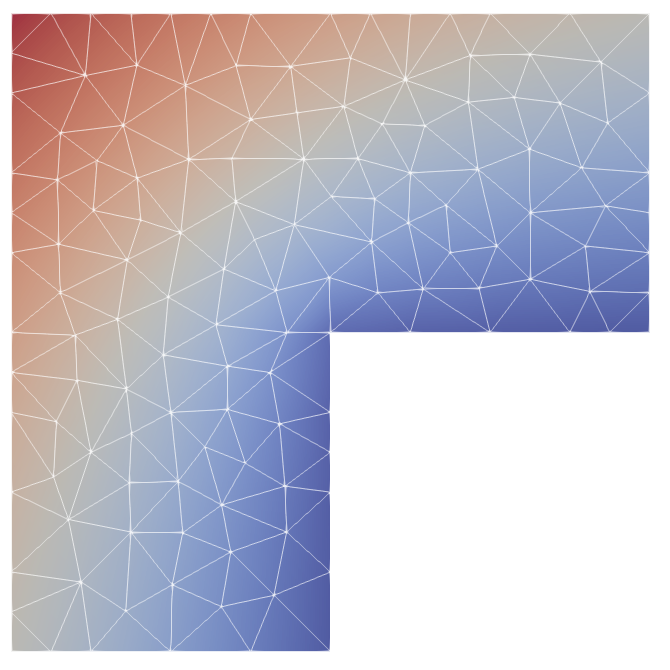
\includegraphics[width=0.4\linewidth]{Images/Test1/h-adaptive/u_initial.png}
  }
     \subfloat[\label{fig:final_mesh} mesh refined after 4 iterations.]{
    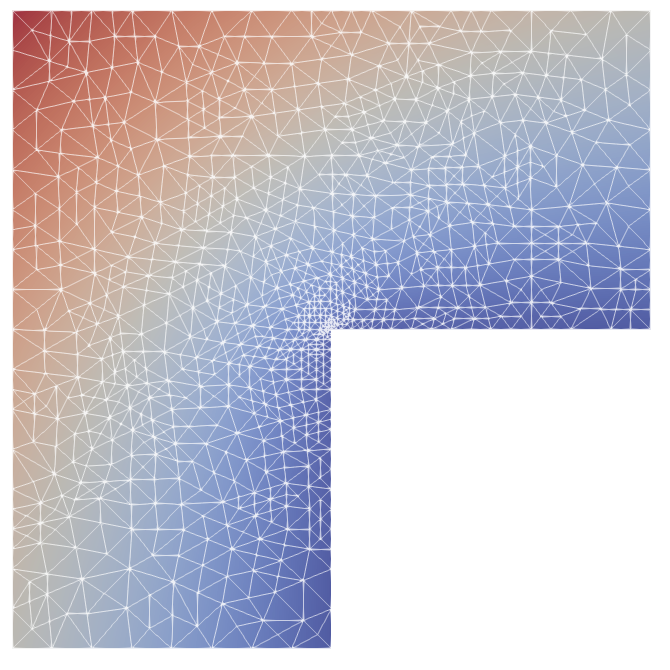
\includegraphics[width=0.4\linewidth]{Images/Test1/h-adaptive/u_final.png}
  }
\caption{Solution of eq.\eqref{eq:poisson_corner} with $h$-refinement ($\hat{\beta} = 0.0$).}
\end{figure}


\begin{figure}[h!]
    \centering
      \subfloat[\label{fig:beta_0.0} $\hat{\beta} = 0.0$.]{
    
\includegraphics[width=0.4\linewidth]{Images/Test1/h-adaptive/u_0.0.png}
  }
     \subfloat[\label{fig:beta_0.33} $\hat{\beta} = 0.33$.]{
    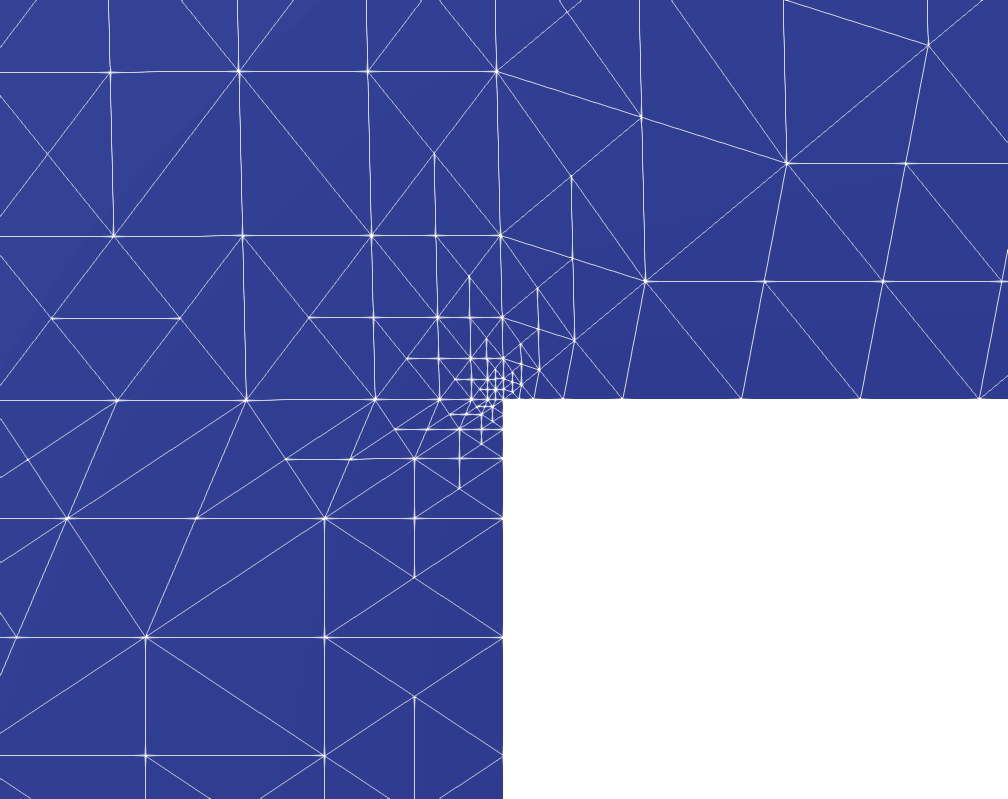
\includegraphics[width=0.4\linewidth]{Images/Test1/h-adaptive/u_0.33.png}
  }\\
      \subfloat[\label{fig:beta_0.5} $\hat{\beta} = 0.5$.]{
    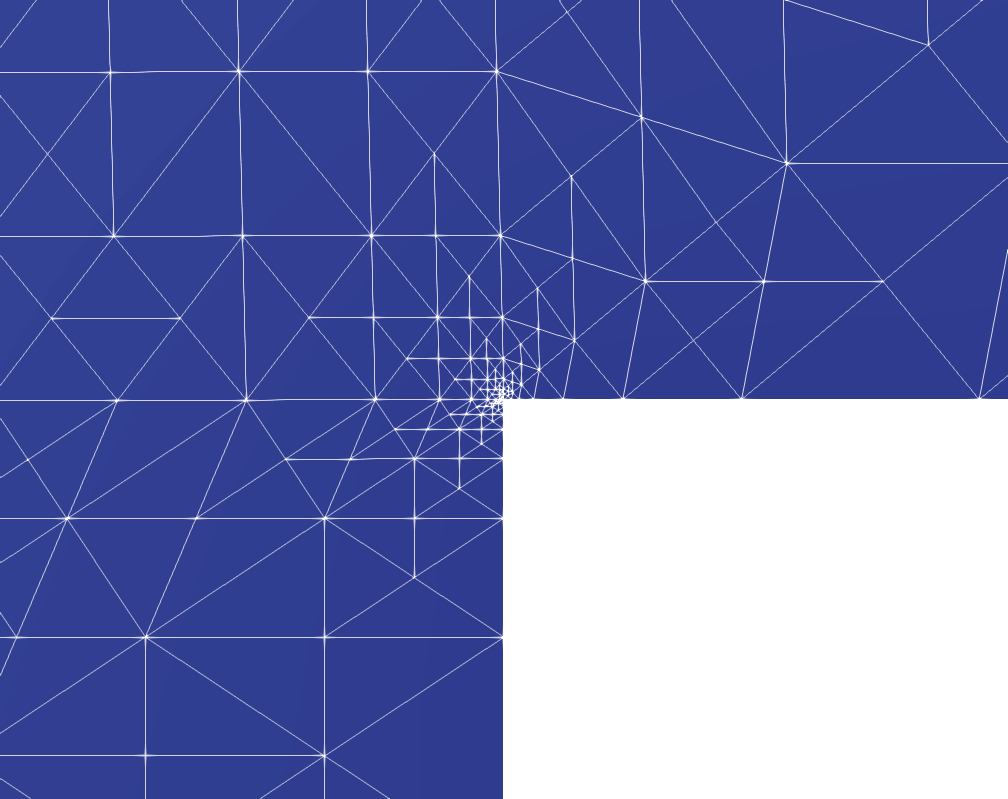
\includegraphics[width=0.4\linewidth]{Images/Test1/h-adaptive/u_0.5.png}
  }
 \subfloat[\label{fig:beta_0.99} $\hat{\beta} = 0.99$.]{
    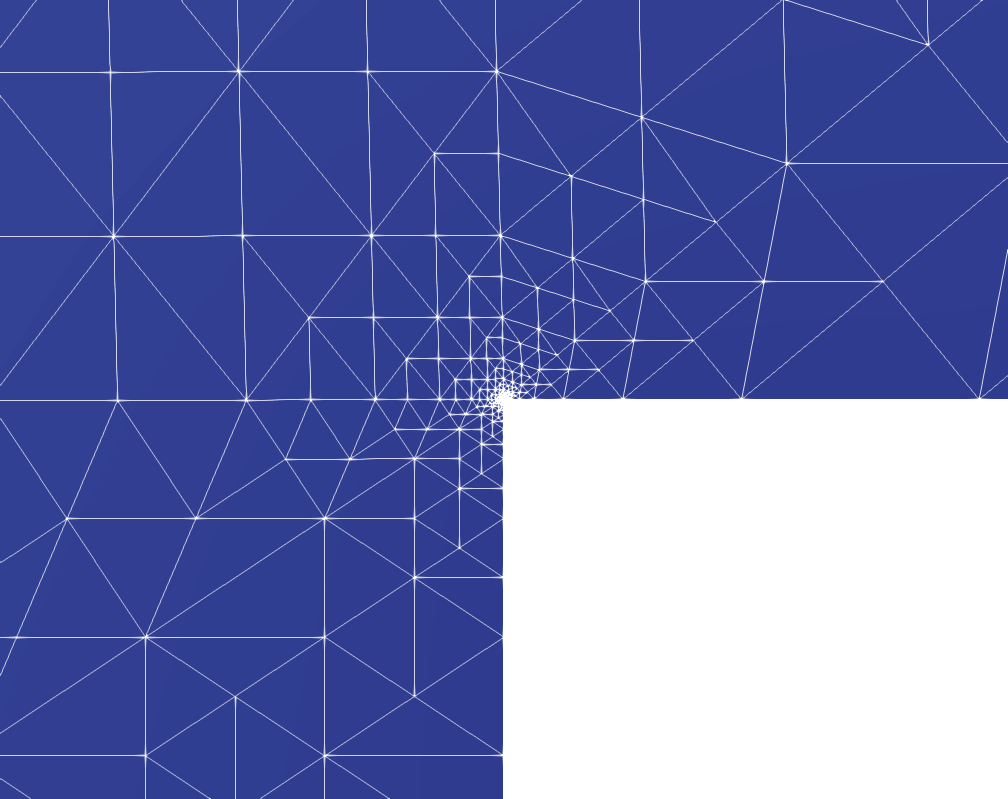
\includegraphics[width=0.4\linewidth]{Images/Test1/h-adaptive/u_0.99.png}
  }
\caption{Solution of eq.\eqref{eq:poisson_corner} near the origin after 14 h-refinements.}
\label{fig:h-ref}
\end{figure}

The \textit{ms} $h$-refinement strategy with $\alpha = 0.1$ has been tested for different $\hat{\beta}$. As visible in Fig.\ref{fig:h-ref}, the level of refinement is increasing near the corner as a function of $\hat{\beta}$. It appears from Fig.\ref{fig:h-ref_rate} that $\hat{\beta} = 0.0$ is already sufficient for achieving an optimal order of convergence.

\subsubsection{a-posteriori bound for $\leb{\infty}$ norm}

An a-posteriori error bound in the $\leb{\infty}$ norm for the SIP-dG method has been derived in \cite{DG:2012}. The domain $\W$ is not required to be Lipschitz, thus the following bound can be tested for our numerical experiments:

\begin{equation}\label{eq:a-posteriori_Linfty}
  \Norm{u-u_{h}}_{\leb{\infty}(\W)} \leq  C l_{h,d} \Big( \Norm{h^{2}(f + \Delta_{h}u_{h})}_{\leb{\infty}(\W)} + \Norm{h \jump{\nabla u_{h}}}_{\leb{\infty}(\cE_{I})} + \Norm{\jump{u_{h}}}_{\leb{\infty}(\cE_{I})} + \Norm{u_{D} - u_{h}}_{\leb{\infty}(\partial \W)} \Big),
\end{equation}

where $l_{h,d} = (\ln frac{1} / \underline{h})^{2}$. 


\subsection{r-adaptive strategy}
\label{sec:r-adaptive}
The r-adaptive strategy aims to generate an adapted mesh $\T{}$ by relocating a fixed number of mesh points. This process can be interpreted as the image from a computational domain $\W_{c}$, having a fixed mesh $\T{}_{c}$, to a physical domain $\W$, with variable mesh $\T{}_{i}$. The first method we propose is a variational one, where the transformation mapping is determined as the minimiser of an adaptation functional \cite{BHR:2009,Winslow:1966}. The Moving Mesh PDE (MMPDE) associated with the minimiser will be solved by the Euler-Lagrange equation.

%A \textit{'radial'} mesh will be also devised, given the a-priori knowledge of radial symmetry of the solution near the corner. The location of the mesh points is obtained by solving a one-dimensional \textit{equidistribution condition} for each straight line spanned from the origin of the domain.

An adaptive mesh based on \textit{Optimal Transport} will be also constructed in the last Subsection \cite{BHR:2009}. This method exploits the strong dependence of the solution on the radial variable, which yields a mesh with high shape regularity and optimal convergence rate. A major advantage of the OT strategy is the computational efficiency, as the adapted mesh is obtained after solving a one dimensional algebraic equation for each node. On the contrary, the implementation of the other r-adaptive methods requires a more computationally expensive iterative procedure. 

\subsubsection{Winslow's diffusion method}
\label{sec:Wins}
The Winslow' diffusion method is defined by the smooth mapping $\vec{x} = (x,y) = \vec{x}(\vec{\xi}) : \W_{c} \rightarrow \W$ or the inverse coordinate
transformation $\vec{\xi} = (\xi,\eta) =  \vec{\xi}(\vec{x}) : \W \rightarrow
\W_{c}$. Practically, most of the MMPDEs were developed in terms of
the inverse coordinate transformation, as this guarantees existence
and uniqueness of the solution \cite{Winslow:1966,Dvinsky:1991}. Thus, we will first solve the MMPDE associated with $\vec{\xi}(\vec{x})$ and the determine the transformed coordinate $\vec{x}(\vec{\xi})$ by change of variable. Consider the functional

\begin{equation}
    I_{Win}[\vec{\xi}] = \frac{1}{2} \int_{\W} \frac{1}{ w(\vec{x})} \sum_{i} (\nabla \xi_{i})^{T} (\nabla \xi_{i}) \d \vec{x},
\label{eq:Winslow_functional_2}
\end{equation}

where $w(\vec{x}) > 0$ is a given monitor function. This function can be chosen to depend on the solution $u_{h}(\vec{x})$ of the physical PDE. We consider as possible choices:

\begin{enumerate}
    \item Gradient:
    
    \begin{equation}
          w|_{K} = \bigg( 1 + \frac{1}{\delta} \, \norm{\nabla_{h} u_{h}}^{2} \bigg)^{1/2}
    \label{eq:monitor_gradient}
    \end{equation}
    
    
    \item Curvature:
    
    \begin{equation}
        w|_{K} = \bigg( 1 +  \frac{1}{\delta} \,\norm{\Delta_{h}u_{h}}\bigg)^{1/2}
    \label{eq:monitor_curvature}
    \end{equation}
    
    \item A-posteriori:  
    
    \begin{equation}
        w|_{K} = \bigg( 1 +  \frac{1}{\delta} \, \eta^{2}_{K}\bigg)^{1/2}
    \label{eq:monitor_posteriori}
    \end{equation}

\end{enumerate}


where $\delta$ is a prescribed intensity parameter for $\T{}$
\cite{HR:2011,BHR:2009}. The MMPDE associated with the functional (\ref{eq:Winslow_functional_2})
becomes
\begin{equation}
  \partial_s \vec{x} (\vec \xi ,s)
  =
  - \sum_{i=1} \vec{a}_{i} \nabla \cdot (\vec M^{-1}\vec{a}^{i}),
\label{eq:MMPDE_Winslow}
\end{equation}

where $s$ denotes the temporal variable, $\vec a^{i} = \nabla \xi_{i}$, $\vec a_{i} = \partial \vec{x}/\partial\xi_{i}$, and $\vec M = w(\vec{x})I_{2}$ is the metric function. The
replacement of the previous terms in the two-dimensional space gives
\begin{equation}
\begin{split}
  \partial_s \vec{x}(\vec{\xi},s)
  =
  \frac{1}{J^{2} w^{2}} \Bigg[& (x_{\eta}^{2} + y_{\eta}^{2})  \frac{\partial}{\partial \xi} \left(w \frac{\partial \vec{x}}{\partial \xi} \right) - (x_{\xi}x_{\eta} + y_{\xi}y_{\eta})\frac{\partial}{\partial \eta} \left( w \frac{\partial \vec{x}}{\partial \xi} \right)\\
      &-(x_{\xi}x_{\eta} + y_{\xi}y_{\eta})\frac{\partial}{\partial \xi} \left(w \frac{\partial \vec{x}}{\partial \eta} \right) + (x_{\xi}^{2} + y_{\xi}^{2})\frac{\partial}{\partial \eta}  \left( w\frac{\partial \vec{x}}{\partial \eta} \right) \Bigg].
\end{split}
\label{eq:MMPDE_Winslow_explicit}
\end{equation}

This PDE allows us to compute $\vec{x}(\vec{\xi},s_{i+1})$ and hence $\T{}_{i+1}$ given the knowledge of $w(\vec{x})$ and $\T{}_{c}$. Equation \eqref{eq:MMPDE_Winslow_explicit} is discretised in space using the FEM with linear Lagrangian elements and in time with the semi-implicit Euler method. To that purpose, we divide the temporal domain $[0,S]$ into a partition of $N_S$ consecutive subintervals $0=s_0 < s_1 < \dots < s_{N_S} = S$ with $s_i - s_{i-1} = k$ for all $i$. We treat the non-linear terms through evaluation at the current time step $s_i$, while the linear terms are evaluated at the next time step $s_{i+1}$.

Dirichlet boundary condition are imposed on all the edges except for that ones intersecting at the re-entrant corner. For those, the monitor function $w(\vec{\xi})$ has been first projected onto the two sides and the solution of the MMPDE5 \cite{HR:2011} in one dimension is computed. This results in the movement of the mesh points towards the origin.\\


The non-convex domain $\W$ poses a practical complication for the application of Winslow's MMPDE. In fact, it is well known that if the computational domain $\W_{c}$ is not convex, the resulting physical mesh might feature very skewed or even overlapping elements. A natural solution for that issue is to define a computational mesh that is convex and solve for the coordinate transformation $\vec{x}(\vec{\xi})$ on this domain \cite{CHR:1999,LTZ:2001}. Once $\W_c$ is selected, a mesh $\T{}_{c}$ with the same topology as $\T{}$ can be constructed by first specifying a correspondence between the boundaries $\partial \W$ and $\partial \W_{c}$ by a mapping $g(\vec{x})$ and then let  $\T{}_{c}$ be the image of $\T{}$ under the mapping $\vec{\xi}(\vec{x})$ satisfying


\begin{equation}
\label{eq:map_domain}
\begin{split}
    \Delta \vec{\xi}(\vec{x}) &= 0 \, \text{ in } \, \W \\
    \vec{\xi} &= g(\vec{x}) \, \text{ on } \, \partial \W.
\end{split}
\end{equation}

\begin{figure}[h!]\label{fig:mesh_Winslow}
    \centering
    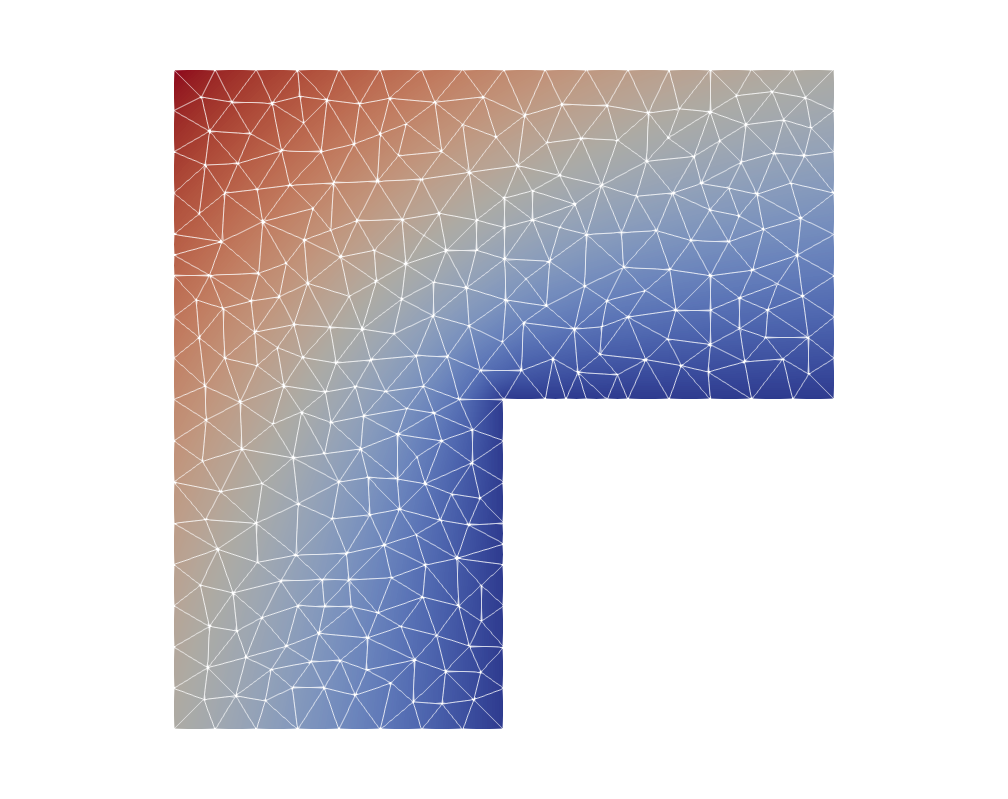
\includegraphics[scale=0.2]{Images/Test1/r-adaptive/u.png}
    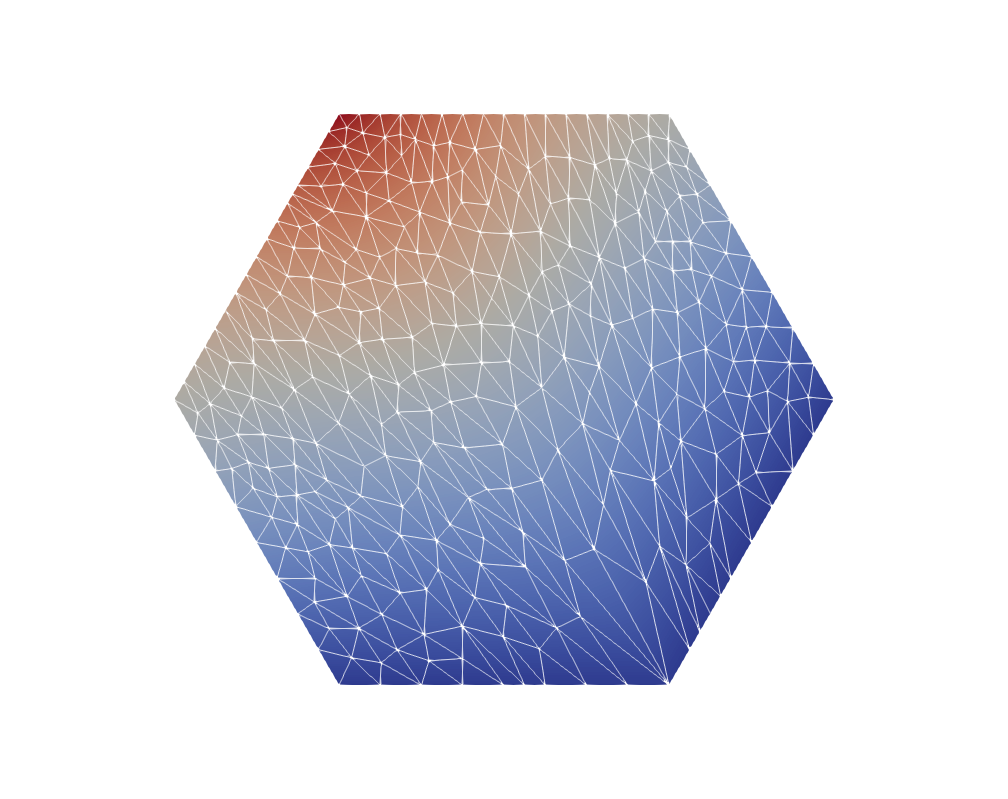
\includegraphics[scale=0.2]{Images/Test1/r-adaptive/u_c.png}
    \caption{Solution of eq.\eqref{eq:poisson_corner} represented in the physical and computational domain.}
    \label{fig:initial_mesh}
\end{figure}

\begin{figure}[h!]
    \centering
    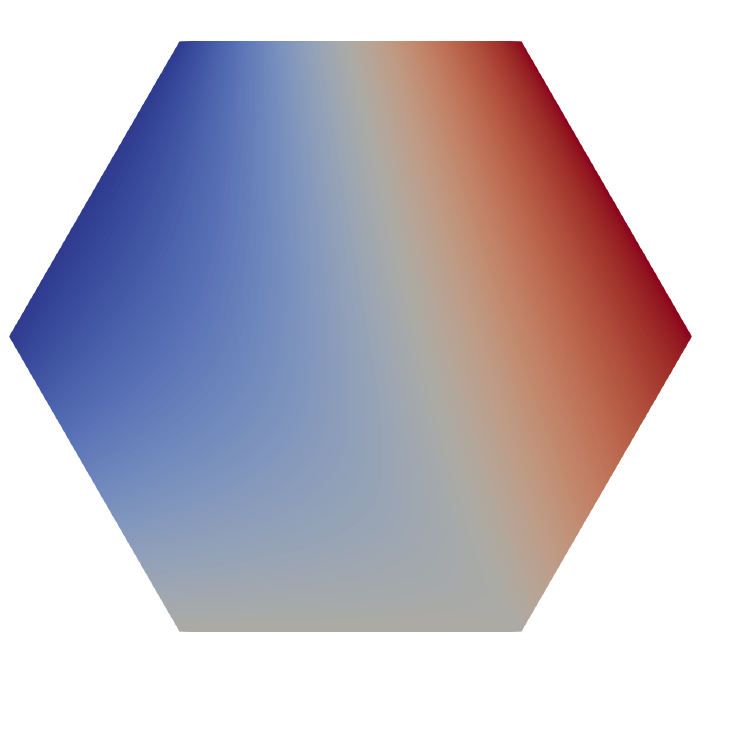
\includegraphics[scale=0.2]{Images/Test1/r-adaptive/xc.png}
    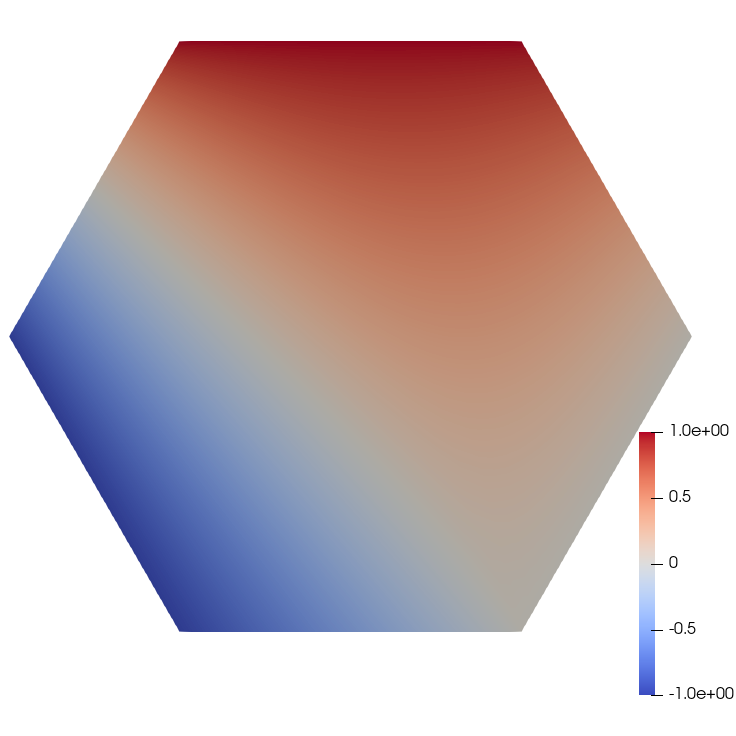
\includegraphics[scale=0.2]{Images/Test1/r-adaptive/yc.png}
    \caption{ $x$ and $y$ coordinates represented in the computational mesh $\T{}_{c}$, obtained as solution of eq.\eqref{eq:map_domain}. The boundary conditions match with that ones of the physical domain.}
    \label{fig:x,y_comp}
\end{figure}
 
\begin{figure}[h!]
    \centering
    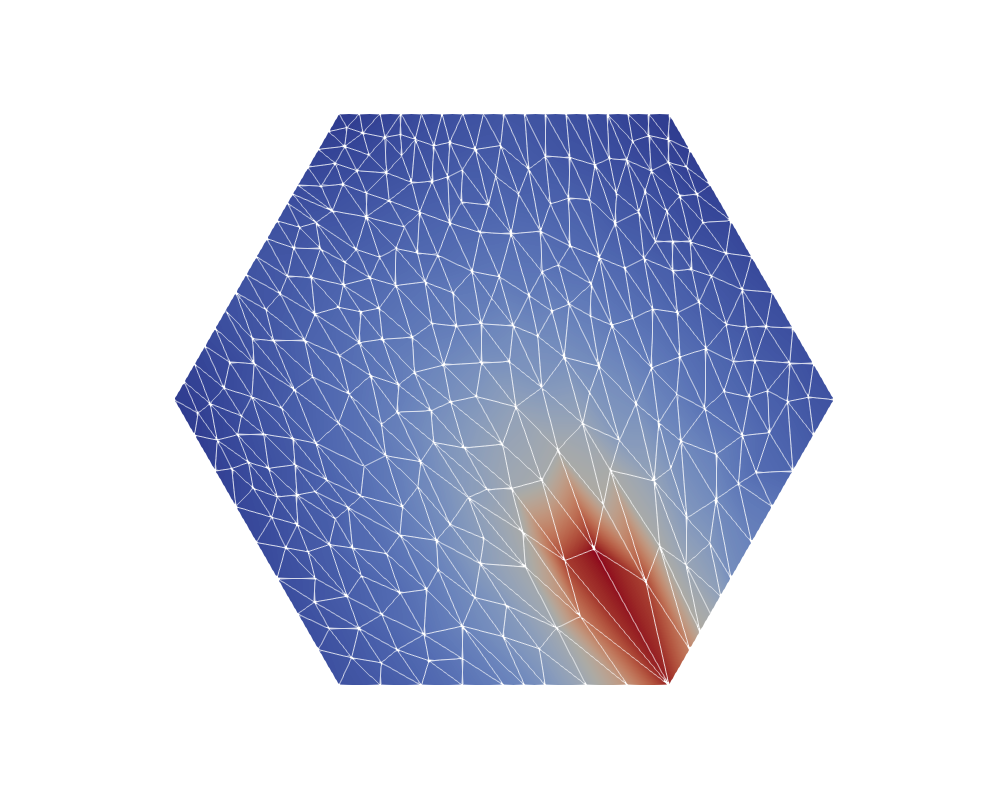
\includegraphics[scale=0.2]{Images/Test1/r-adaptive/w_c.png}
    \caption{Monitor function $w(\vec{\xi})$ in the computational domain.}
    \label{fig:monitor_comp}
  \end{figure}

%\subsubsection{Radial mesh}
%The 'radial' mesh is obtained by solving the one-dimensional equidistribution condition 

%\begin{equation}
%   \rho(x)\frac{d x}{d \xi} = \sigma, \quad  \xi \in [0,1], \, x \in [0,L_{i}], \, i = 0,\dots,N,
%\label{eq:1D_equid}
%\end{equation}

%where $\sigma = \int_{a}^{b}\rho(x) d x$ and $L_{i}$ represents the length of the line $l_{i}$ spanning from the origin with slope angle $\theta_{i} = i d \theta $ so that $\theta_{N} = \frac{3\pi}{2}$. The angle width $d \theta$ is chosen such that the number of lines is equal to the number of mesh nodes along each of them. The monitor function $\rho$ is computed accordingly to \cite{HR:2011} as:

%\begin{equation}
%\rho = \left( 1 + \frac{1}{\alpha}  |u'|^{2} \right)^{1/3}, \quad \alpha = \left[ \int_{0}^{1}  |u'|^{2/3} \ dx \right]^{3}
%\label{eq:optimal_rho}
%\end{equation}

%Equation \eqref{eq:1D_equid} is solved numerically by using \textit{De Boor'} algorithm with the Finite Difference method \cite{XHWW:2011} until reaching convergence, with relative tolerance fixed to $10^{-8}$. 

\begin{figure}[h!]\label{fig:r-adaptive_meshes}
    \centering
      \subfloat[\label{fig:u_gradient} Mesh adapted with gradient monitor function.]{
    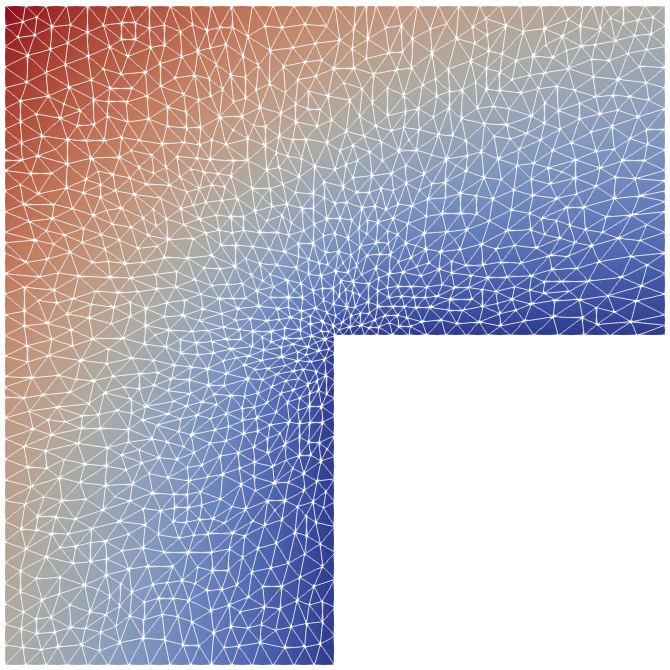
\includegraphics[width=0.4\linewidth]{Images/Test1/r-adaptive/u_gradient.png}
  }
     \subfloat[\label{fig:u_curvature} Mesh adapted with curvature monitor function.]{
    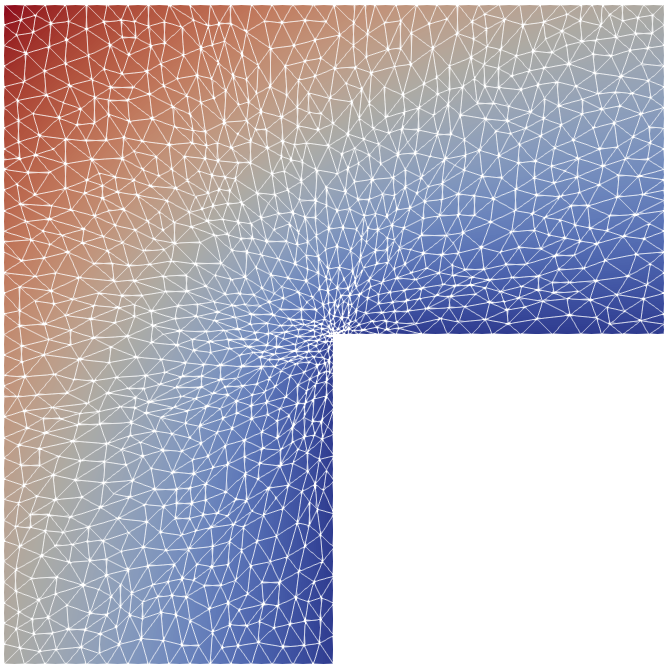
\includegraphics[width=0.4\linewidth]{Images/Test1/r-adaptive/u_curvature.png}
  }\\
      \subfloat[\label{fig:u_posteriori_0.0} Mesh adapted with a-posteriori monitor function ($\hat{\beta} = 0.0$).]{
    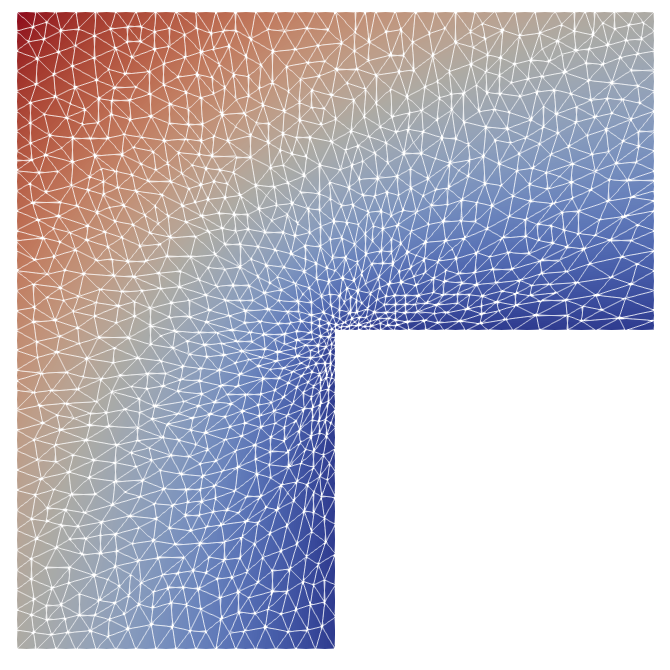
\includegraphics[width=0.4\linewidth]{Images/Test1/r-adaptive/u_posteriori_0.99.png}
  }
 \subfloat[\label{fig:u_posteriori_0.99}Mesh adapted with a-posteriori monitor function ($\hat{\beta} = 0.99$).]{
    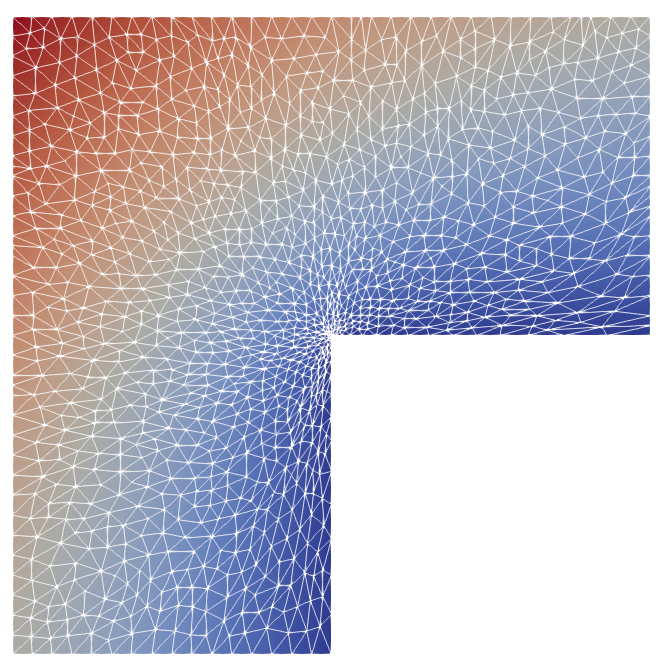
\includegraphics[width=0.4\linewidth]{Images/Test1/r-adaptive/u_posteriori_0.0.png}
  }
\caption{Solution of eq.\eqref{eq:poisson_corner} with Winslow's MMPDE for different monitor functions with $\dim \fes = 7005$.}
\label{fig:adapted_mesh}
\end{figure}


\begin{figure}[h!]\label{tixz:conv_rate_r-adaptive}
\centering
\begin{tikzpicture}
  \begin{axis}[
      cycle list/Dark2,
      thick,
      xmode=log,
      ymode=log,
      xlabel=$\dim \fes$,
      ylabel=$\Norm{u - u_{h}}_{\leb{2}(\W)}$,
      grid=both,
      minor grid style={gray!25},
      major grid style={gray!25},
      width=0.48\linewidth,
      %no marks,
     legend style={at={(0.0,0.0)},anchor=south west},
    ]
%\addplot+[color=yellow,mark = +]
%	table[x=dof,y=error, col sep=comma]{Data/Test1/radial/radial.csv};
%\addlegendentry{radial};
\addplot+[color=black,mark = triangle]
	table[x=dof,y=error, col sep=comma]{Data/Test1/uniform/uniform.csv};
\addlegendentry{uniform};
\addplot+[color=green, mark = star]
	table[x=dof,y=error, col sep=comma]{Data/Test1/r-adaptive/gradient/gradient.csv};
\addlegendentry{gradient};
\addplot+[color=orange, mark = square]
	table[x=dof,y=error, col sep=comma]{Data/Test1/r-adaptive/curvature/curvature.csv};
\addlegendentry{curvature};
\addplot+[color=cyan, mark = star]
	table[x=dof,y=error, col sep=comma]{Data/Test1/r-adaptive/a-posteriori/beta_0.0/posteriori_rate.csv};
%\addlegendentry{$\hat{\beta} = 0.0$};
%\addplot+[color=blue, mark = star]
%	table[x=dof,y=error, col sep=comma]{Data/Test1/r-adaptive/a-posteriori/beta_0.33/posteriori_rate.csv};
%\addlegendentry{$\hat{\beta} = 0.33$};
%\addplot+[color=purple, mark = star]
%	table[x=dof,y=error, col sep=comma]{Data/Test1/r-adaptive/a-posteriori/beta_0.5/posteriori_rate.csv};
%\addlegendentry{$\hat{\beta} = 0.5$};
%\addplot+[color=red, mark = star]
%	table[x=dof,y=error, col sep=comma]{Data/Test1/r-adaptive/a-posteriori/beta_0.99/posteriori_rate.csv};
\addlegendentry{$\hat{\beta} = 0.99$};
\draw[thick,black] (30000,0.00004) -- (80000,0.00004) -- (30000,0.000107)--cycle;
\node at (40000,0.00005) {$1.0$};
\draw[thick,black] (30000,0.000385859365913) -- (80000,0.000385859365913) -- (80000,0.0002)--cycle;
\node at (120000,0.00032) {$0.67$};
\end{axis}
\end{tikzpicture}
\caption{Asymptotic convergence rates of Winslow's MMPDE for different monitor functions $w$ \eqref{eq:monitor_gradient}-\eqref{eq:monitor_posteriori}.}
\end{figure}

\begin{figure}[h!]
  \subfloat[{\label{fig:1-a}}
    MMPDE with gradient monitor function.]{
\begin{tikzpicture}
  \begin{axis}[
      cycle list/Dark2,
      thick,
      xmode=linear,
      ymode=log,
      xlabel=$i$,
      ylabel=$\Norm{u - u_{h}}_{\leb{2}(\W)}$,
      grid=both,
      minor grid style={gray!25},
      major grid style={gray!25},
      width=0.38\linewidth,
      %no marks,
      %legend style={at={(0.0,0.15)},anchor=north east},
    ]
\addplot+[mark=star]
	table[x=iteration,y=error, col sep=comma]{Data/Test1/r-adaptive/gradient/gradient_684.csv};
%\addlegendentry{dof 1};
\addplot+[mark=star]
	table[x=iteration,y=error, col sep=comma]{Data/Test1/r-adaptive/gradient/gradient_1716.csv};
%\addlegendentry{dof 2};
\addplot+[mark=star]
	table[x=iteration,y=error, col sep=comma]{Data/Test1/r-adaptive/gradient/gradient_7005.csv};
%\addlegendentry{dof 3};
\addplot+[mark=star]
	table[x=iteration,y=error, col sep=comma]{Data/Test1/r-adaptive/gradient/gradient_28290.csv};
%\addlegendentry{dof 4};
\addplot+[mark=star]
	table[x=iteration,y=error, col sep=comma]{Data/Test1/r-adaptive/gradient/gradient_100080.csv};
%\addlegendentry{dof 5};
\end{axis}
\end{tikzpicture}
}
\subfloat[{\label{fig:1-b}}
MMPDE with curvature monitor function.
]
{
\begin{tikzpicture}
  \begin{axis}[
      cycle list/Dark2,
      thick,
      xmode=linear,
      ymode=log,
      xlabel=$i$,
      grid=both,
      minor grid style={gray!25},
      major grid style={gray!25},
      width=0.38\linewidth,
      %no marks,
      ylabel near ticks,
      %yticklabel pos=right,
      %legend style={at={(0,1)},anchor=north west},
    ]
\addplot+[mark=star]
	table[x=iteration,y=error, col sep=comma]{Data/Test1/r-adaptive/curvature/curvature_684.csv};
\addlegendentry{dof 1};
\addplot+[mark=star]
	table[x=iteration,y=error, col sep=comma]{Data/Test1/r-adaptive/curvature/curvature_1716.csv};
\addlegendentry{dof 2};
\addplot+[mark=star]
	table[x=iteration,y=error, col sep=comma]{Data/Test1/r-adaptive/curvature/curvature_7005.csv};
\addlegendentry{dof 3};
\addplot+[mark=star]
	table[x=iteration,y=error, col sep=comma]{Data/Test1/r-adaptive/curvature/curvature_28290.csv};
\addlegendentry{dof 4};
\addplot+[mark=star]
	table[x=iteration,y=error, col sep=comma]{Data/Test1/r-adaptive/curvature/curvature_100080.csv};
\addlegendentry{dof 5};
\end{axis}
\end{tikzpicture}
}
\subfloat[{\label{fig:1-c}}
MMPDE with a-posteriori monitor function ($\hat{\beta} = 0.0$).
  ]{
\begin{tikzpicture}
  \begin{axis}[
      cycle list/Dark2,
      thick,
      xmode=linear,
      ymode=log,
      xlabel=$i$,
      ylabel=$\Norm{u - u_{h}}_{\leb{2}(\W)}$,
      grid=both,
      minor grid style={gray!25},
      major grid style={gray!25},
      width=0.38\linewidth,
      %no marks,
      %legend style={at={(0.0,0.15)},anchor=north east},
    ]
\addplot+[mark=star]
	table[x=iteration,y=error, col sep=comma]{Data/Test1/r-adaptive/a-posteriori/beta_0.0/posteriori_684.csv};
%\addlegendentry{dof 1};
\addplot+[mark=star]
	table[x=iteration,y=error, col sep=comma]{Data/Test1/r-adaptive/a-posteriori/beta_0.0/posteriori_1716.csv};
%\addlegendentry{dof 2};
\addplot+[mark=star]
	table[x=iteration,y=error, col sep=comma]{Data/Test1/r-adaptive/a-posteriori/beta_0.0/posteriori_7005.csv};
%\addlegendentry{dof 3};
\addplot+[mark=star]
	table[x=iteration,y=error, col sep=comma]{Data/Test1/r-adaptive/a-posteriori/beta_0.0/posteriori_28290.csv};
%\addlegendentry{dof 4};
\addplot+[mark=star]
	table[x=iteration,y=error, col sep=comma]{Data/Test1/r-adaptive/a-posteriori/beta_0.0/posteriori_100080.csv};
%\addlegendentry{dof 5};
\end{axis}
\end{tikzpicture}
}
\subfloat[{\label{fig:1-d}}
    MMPDE with a-posteriori monitor function ($\hat{\beta} = 0.33$).
]
{
\begin{tikzpicture}
  \begin{axis}[
      cycle list/Dark2,
      thick,
      xmode=linear,
      ymode=log,
      xlabel=$i$,
      grid=both,
      minor grid style={gray!25},
      major grid style={gray!25},
      width=0.4\linewidth,
      %no marks,
      ylabel near ticks,
      yticklabel pos=right,
      %legend style={at={(0,1)},anchor=north west},
    ]
\addplot+[mark=star]
	table[x=iteration,y=error, col sep=comma]{Data/Test1/r-adaptive/a-posteriori/beta_0.33/posteriori_684.csv};
\addlegendentry{dof 1};
\addplot+[mark=star]
	table[x=iteration,y=error, col sep=comma]{Data/Test1/r-adaptive/a-posteriori/beta_0.33/posteriori_1716.csv};
\addlegendentry{dof 2};
\addplot+[mark=star]
	table[x=iteration,y=error, col sep=comma]{Data/Test1/r-adaptive/a-posteriori/beta_0.33/posteriori_7005.csv};
\addlegendentry{dof 3};
\addplot+[mark=star]
	table[x=iteration,y=error, col sep=comma]{Data/Test1/r-adaptive/a-posteriori/beta_0.33/posteriori_28290.csv};
\addlegendentry{dof 4};
\addplot+[mark=star]
	table[x=iteration,y=error, col sep=comma]{Data/Test1/r-adaptive/a-posteriori/beta_0.33/posteriori_100080.csv};
\addlegendentry{dof 5};
%\addlegendentry{Discontinuous (\ref{eq:discontinuous})};
\end{axis}
\end{tikzpicture}
}\\
\subfloat[{\label{fig:1-e}}
    MMPDE with a-posteriori monitor function ($\hat{\beta} = 0.5$).
]
{
\begin{tikzpicture}
  \begin{axis}[
      cycle list/Dark2,
      thick,
      xmode=linear,
      ymode=log,
      xlabel=$i$,
      ylabel = $\Norm{u - u_{h}}_{\leb{2}(\W)}$,
      grid=both,
      minor grid style={gray!25},
      major grid style={gray!25},
      width=0.38\linewidth,
      %no marks,
      ylabel near ticks,
      yticklabel pos=left,
      %legend style={at={(0,1)},anchor=north west},
    ]
\addplot+[mark=star]
	table[x=iteration,y=error, col sep=comma]{Data/Test1/r-adaptive/a-posteriori/beta_0.5/posteriori_684.csv};
%\addlegendentry{dof 1};
\addplot+[mark=star]
	table[x=iteration,y=error, col sep=comma]{Data/Test1/r-adaptive/a-posteriori/beta_0.5/posteriori_1716.csv};
%\addlegendentry{dof 2};
\addplot+[mark=star]
	table[x=iteration,y=error, col sep=comma]{Data/Test1/r-adaptive/a-posteriori/beta_0.5/posteriori_7005.csv};
%\addlegendentry{dof 3};
\addplot+[mark=star]
	table[x=iteration,y=error, col sep=comma]{Data/Test1/r-adaptive/a-posteriori/beta_0.5/posteriori_28290.csv};
%\addlegendentry{dof 4};
\addplot+[mark=star]
	table[x=iteration,y=error, col sep=comma]{Data/Test1/r-adaptive/a-posteriori/beta_0.5/posteriori_100080.csv};
%\addlegendentry{dof 5};
%\addlegendentry{Discontinuous (\ref{eq:discontinuous})};
\end{axis}
\end{tikzpicture}
}
\subfloat[{\label{fig:1-f}}
    MMPDE with a-posteriori monitor function ($\hat{\beta} = 0.99$).
]
{
\begin{tikzpicture}
  \begin{axis}[
      cycle list/Dark2,
      thick,
      xmode=linear,
      ymode=log,
      xlabel=$i$,
      grid=both,
      minor grid style={gray!25},
      major grid style={gray!25},
      width=0.38\linewidth,
      %no marks,
      ylabel near ticks,
      yticklabel pos=left,
      %legend style={at={(0,1)},anchor=north west},
    ]
\addplot+[mark=star]
	table[x=iteration,y=error, col sep=comma]{Data/Test1/r-adaptive/a-posteriori/beta_0.99/posteriori_684.csv};
%\addlegendentry{dof 1};
\addplot+[mark=star]
	table[x=iteration,y=error, col sep=comma]{Data/Test1/r-adaptive/a-posteriori/beta_0.99/posteriori_1716.csv};
%\addlegendentry{dof 2};
\addplot+[mark=star]
	table[x=iteration,y=error, col sep=comma]{Data/Test1/r-adaptive/a-posteriori/beta_0.99/posteriori_7005.csv};
%\addlegendentry{dof 3};
\addplot+[mark=star]
	table[x=iteration,y=error, col sep=comma]{Data/Test1/r-adaptive/a-posteriori/beta_0.99/posteriori_28290.csv};
%\addlegendentry{dof 4};
\addplot+[mark=star]
	table[x=iteration,y=error, col sep=comma]{Data/Test1/r-adaptive/a-posteriori/beta_0.99/posteriori_100080.csv};
%\addlegendentry{dof 5};
%\addlegendentry{Discontinuous (\ref{eq:discontinuous})};
\end{axis}
\end{tikzpicture}}
\caption{The solution error decreases monotonically over the iterations until reaching convergence for all the monitor functions. The relative tolerance has been fixed to $1\times10^{-5}$, while the timestep has been set to $k=10^{-3}$. The degrees of freedom in the legend are $684$, $1716$, $7005$, $28290$, and $100080$.}
\end{figure}

\clearpage
\newpage

\subsubsection{Optimal Transport mesh}
\label{sec:OT}

We devise a mesh for the L-shaped region by solving the Monge-Ampère equation close to the re-entrant corner. The solution is then tuned to match the boundary of the domain.


\paragraph{Local mesh scaling}

Consider the general solution of equation \eqref{eq:poisson_corner}. We know that the interpolation error of the solution for piecewise linear element can be bounded in the $\leb{2}$ norm by $E_{max} \sim h^{2} r^{\pi/\omega - 2}$, where $h$ is the local mesh size of an element close to the corner and r is the distance from the re-entrant corner, placed at the origin of $\reals^{2}$.\\

Following the \textit{equidistribution principle}, we impose $E_{max} = 1$, so that we obtain $h \sim r^{\gamma}$, where $\gamma = 1 - \frac{\pi}{2\omega}$. Given the computation variable $s$, which represent the distance from the origin in the computational domain $\W_{c} \equiv \W$, we can interpret $h$ as being proportional to $dr/ds$. Solving the differential equation $\frac{dr}{ds} = h = r^{\gamma}$ we obtain that $r \sim s^{\frac{1}{1-\gamma}}$.


\paragraph{Solution of Monge-Ampère equation}
\label{sec:sol_MA}
We now look for a radially symmetric transformation from the corner region to itself. We can assume a radial symmetry because the singular behaviour of the solution near the origin does not depend on the angle $\theta$. More details on the application of approach can be found in \cite{BRW:2015}. Locally, the first integral of the Monge-Ampère equation implies that $r$ satisfies the Ordinary Differential Equation (ODE) in polar coordinates

\begin{equation}
    m(r)r \, dr d\theta = s \, ds d\theta,
\label{eq:Monge-Ampere}
\end{equation}

where $m(r) = r^{-2 \gamma}$ is the monitor function, which will be determined by the \textit{a-priori} estimate for the interpolation error.

We expect that for large $r$ the adapted mesh is almost regular. we then expect that $m(r) \sim 1$ far from the corner and consider the general expression 

\begin{equation}
    m(r) = A + B r^{-2 \gamma}, \quad \alpha,\beta \in \reals
\end{equation}


From \eqref{eq:Monge-Ampere} we integrate over the variable $\theta$ and obtain

$$\left(A + B r^{-2\gamma}\right) r \frac{dr}{ds} = s,$$

so that $r$ satisfies the nonlinear algebraic equation 

\begin{equation}
    A r^{2} + \frac{B}{1-\gamma}r^{2(1-\gamma)} = s^{2}.
\label{eq:mesh_transformation}
\end{equation}

The equation \eqref{eq:mesh_transformation} then determines the mesh transformation. Note that the parameter $A$ and $B$ controls the level of mesh compression near the corner. In fact, for high values of $B$ and small $r$ we have $r \sim s^{1/(1-\gamma)}$ and for large $A$ and $r$ we have $r \sim s$. For the remainder of the analysis, we choose $B = (1-\gamma)$, as this is the maximum admissible value that respects the boundary condition $A + B/(1-\gamma) = 1$ when $r,s = 1$. 


\paragraph{Computation of the OT mesh}

Suppose we have a uniform regular mesh $(\xi_{i,j},\eta_{i,j})$ in $\W_{c}$ which we want to map to an adapted non uniform mesh $(x_{i,j},y_{i,j})$ in the physical domain, with $i,j = 1,\dots,N$. The application of the Monge-Ampère method provides the desired mesh as follows:

\begin{enumerate}
    \item For each pair $(i,j)$ compute $s_{i,j}^{2} = \xi_{i,j}^{2} + \eta_{i,j}^{2}$
    \item Compute the angle $\theta_{i,j}$ with respect to the semi-positive $x$ axis by $\arctan{\frac{\eta_{i,j}}{\xi_{i,j}}}$. 
    \item Compute the length $l_{i,j}$ of the line spanned from the origin with angle $\theta_{i,j}$ to the boundary of the L-shaped domain.
    \item Set the parameter $B = 1 - \gamma$ and enforce the condition $A + \frac{B}{1-\gamma}l_{i,j}^{-2\gamma} = 1$. This ensures that the new mesh boundary matches with the original boundary region.
      
    \item Solve equation \eqref{eq:mesh_transformation} to find $r_{i,j}$
    \item Set $(x_{i,j},y_{i,j}) = \frac{r_{i,j}}{s_{i,j}}(\xi_{i,j},\eta_{i,j})$.
\end{enumerate}


Given the new mesh $(x_{i,j},y_{i,j})$, we can increase the dofs by uniform refinement or by applying the previous procedure from a more graded uniform mesh. The first approach is less computationally expensive and provides higher accuracy.


\paragraph{OT mesh for different $\gamma$}

In this Section, we show how the parameter $\gamma$ affects the accuracy and the quality of the resulting OT mesh. 


\begin{figure}[h!]\label{tikz:OT_gamma_error}
\centering
\subfloat[{\label{fig:error_gamma_L2}} $\leb{2}$ error for different $\gamma$]{  
\begin{tikzpicture}
  \begin{axis}[
      cycle list/Dark2,
      thick,
      xmode=log,
      ymode=log,
      xlabel=$\dim \fes$,
      ylabel=$\Norm{u - u_{h}}_{\leb{2}(\W)}$,
      grid=both,
      minor grid style={gray!25},
      major grid style={gray!25},
      width=0.5\linewidth,
      %no marks,
      legend style={at={(0.0,0.0)},anchor=south west},
    ]
\addplot+[color=black,mark = triangle]
        table[x=dof,y=error, col sep=comma]{Data/Test1/OT/a_priori/errorL2_0.0.csv};
\addlegendentry{$\gamma = 0.0$};
\addplot+[color=red,mark = triangle]
	table[x=dof,y=error, col sep=comma]{Data/Test1/OT/a_priori/errorL2_0.2.csv};
\addlegendentry{$\gamma = 0.2$};
\addplot+[color=green,mark = triangle]
	table[x=dof,y=error, col sep=comma]{Data/Test1/OT/a_priori/errorL2_0.33.csv};
\addlegendentry{$\gamma = 0.33$};        
\addplot+[color=blue,mark = triangle]
	table[x=dof,y=error, col sep=comma]{Data/Test1/OT/a_priori/errorL2_0.53.csv};
\addlegendentry{$\gamma = 0.53$};
\addplot+[color=cyan,mark = triangle]
	table[x=dof,y=error, col sep=comma]{Data/Test1/OT/a_priori/errorL2_0.67.csv};
\addlegendentry{$\gamma = 0.67$};
\addplot+[color=magenta,mark = triangle]
        table[x=dof,y=error, col sep=comma]{Data/Test1/OT/a_priori/errorL2_0.8.csv};
\addlegendentry{$\gamma = 0.8$};
\addplot+[color=yellow,mark = triangle]
	table[x=dof,y=error, col sep=comma]{Data/Test1/OT/a_priori/errorL2_0.9.csv};
\addlegendentry{$\gamma = 0.9$};        
\end{axis}
\end{tikzpicture}
}
\subfloat[{\label{fig:error_gamma_Linfty}} $\leb{\infty}$ error for different $\gamma$]{  
\begin{tikzpicture}
  \begin{axis}[
      cycle list/Dark2,
      thick,
      xmode=log,
      ymode=log,
      xlabel=$\dim \fes$,
      ylabel=$\Norm{u - u_{h}}_{\leb{\infty}(\W)}$,
      grid=both,
      minor grid style={gray!25},
      major grid style={gray!25},
      width=0.5\linewidth,
      %no marks,
      %legend style={at={(0.0,0.0)},anchor=south west},
    ]
\addplot+[color=black,mark = triangle]
        table[x=dof,y=error, col sep=comma]{Data/Test1/OT/a_priori/errorLinfty_0.0.csv};
%\addlegendentry{$\gamma = 0.0$};
\addplot+[color=red,mark = triangle]
	table[x=dof,y=error, col sep=comma]{Data/Test1/OT/a_priori/errorLinfty_0.2.csv};
%\addlegendentry{$\gamma = 0.2$};
\addplot+[color=green,mark = triangle]
	table[x=dof,y=error, col sep=comma]{Data/Test1/OT/a_priori/errorLinfty_0.33.csv};
%\addlegendentry{$\gamma = 0.33$};        
\addplot+[color=blue,mark = triangle]
	table[x=dof,y=error, col sep=comma]{Data/Test1/OT/a_priori/errorLinfty_0.53.csv};
%\addlegendentry{$\gamma = 0.53$};
\addplot+[color=cyan,mark = triangle]
	table[x=dof,y=error, col sep=comma]{Data/Test1/OT/a_priori/errorLinfty_0.67.csv};
%\addlegendentry{$\gamma = 0.67$};
\addplot+[color=magenta,mark = triangle]
        table[x=dof,y=error, col sep=comma]{Data/Test1/OT/a_priori/errorLinfty_0.8.csv};
%\addlegendentry{$\gamma = 0.8$};
\addplot+[color=yellow,mark = triangle]
	table[x=dof,y=error, col sep=comma]{Data/Test1/OT/a_priori/errorLinfty_0.9.csv};
%\addlegendentry{$\gamma = 0.9$};        
\end{axis}
\end{tikzpicture}
}\\
\subfloat[{\label{fig:q_gamma}} mesh condition of OT mesh for different $\gamma$]{  
\begin{tikzpicture}
  \begin{axis}[
      cycle list/Dark2,
      thick,
      xmode=log,
      ymode=log,
      xlabel=$\dim \fes$,
      ylabel=$q$,
      grid=both,
      minor grid style={gray!25},
      major grid style={gray!25},
      width=0.5\linewidth,
      %no marks,
      %legend style={at={(0.1,0.1)},anchor=south west},
    ]
%\addplot+[color=black,mark = triangle]
%        table[x=dof,y=q, col sep=comma]{Data/Test1/OT/a_priori/stat_0.0.csv};
%\addlegendentry{$\gamma = 0.0$};
\addplot+[color=red,mark = triangle]
	table[x=dof,y=q, col sep=comma]{Data/Test1/OT/a_priori/stat_0.2.csv};
%\addlegendentry{$\gamma = 0.2$};
\addplot+[color=green,mark = triangle]
	table[x=dof,y=q, col sep=comma]{Data/Test1/OT/a_priori/stat_0.33.csv};
%\addlegendentry{$\gamma = 0.33$};        
\addplot+[color=blue,mark = triangle]
	table[x=dof,y=q, col sep=comma]{Data/Test1/OT/a_priori/stat_0.53.csv};
%\addlegendentry{$\gamma = 0.53$};
\addplot+[color=cyan,mark = triangle]
	table[x=dof,y=q, col sep=comma]{Data/Test1/OT/a_priori/stat_0.67.csv};
%\addlegendentry{$\gamma = 0.67$};
\addplot+[color=magenta,mark = triangle]
        table[x=dof,y=q, col sep=comma]{Data/Test1/OT/a_priori/stat_0.8.csv};
%\addlegendentry{$\gamma = 0.8$};
\addplot+[color=yellow,mark = triangle]
	table[x=dof,y=q, col sep=comma]{Data/Test1/OT/a_priori/stat_0.9.csv};
%\addlegendentry{$\gamma = 0.9$};        
\end{axis}
\end{tikzpicture}
}
\subfloat[{\label{fig:mu_gamma}} shape regularity for different $\gamma$]{  
\begin{tikzpicture}
  \begin{axis}[
      cycle list/Dark2,
      thick,
      xmode=log,
      ymode=log,
      xlabel=$\dim \fes$,
      ylabel=$\mu$,
      grid=both,
      minor grid style={gray!25},
      major grid style={gray!25},
      width=0.5\linewidth,
      %no marks,
      %legend style={at={(0.1,0.1)},anchor=south west},
    ]
%\addplot+[color=black,mark = triangle]
%        table[x=dof,y=mu, col sep=comma]{Data/Test1/OT/a_priori/stat_0.0.csv};
%\addlegendentry{$\gamma = 0.0$};
\addplot+[color=red,mark = triangle]
	table[x=dof,y=mu, col sep=comma]{Data/Test1/OT/a_priori/stat_0.2.csv};
%\addlegendentry{$\gamma = 0.2$};
\addplot+[color=green,mark = triangle]
	table[x=dof,y=mu, col sep=comma]{Data/Test1/OT/a_priori/stat_0.33.csv};
%\addlegendentry{$\gamma = 0.33$};        
\addplot+[color=blue,mark = triangle]
	table[x=dof,y=mu, col sep=comma]{Data/Test1/OT/a_priori/stat_0.53.csv};
%\addlegendentry{$\gamma = 0.53$};
\addplot+[color=cyan,mark = triangle]
	table[x=dof,y=mu, col sep=comma]{Data/Test1/OT/a_priori/stat_0.67.csv};
%\addlegendentry{$\gamma = 0.67$};
\addplot+[color=magenta,mark = triangle]
        table[x=dof,y=mu, col sep=comma]{Data/Test1/OT/a_priori/stat_0.8.csv};
%\addlegendentry{$\gamma = 0.8$};
\addplot+[color=yellow,mark = triangle]
	table[x=dof,y=mu, col sep=comma]{Data/Test1/OT/a_priori/stat_0.9.csv};
%\addlegendentry{$\gamma = 0.9$};        
\end{axis}
\end{tikzpicture}
}
\caption{Error and quality measure of the OT mesh for different $\gamma$.}
\end{figure}


\begin{figure}
\centering
\subfloat[{\label{fig:L2_gamma}} Error as function of $\gamma$]{  
\begin{tikzpicture}
  \begin{axis}[
      cycle list/Dark2,
      thick,
      xmode=log,
      ymode=log,
      xlabel=$\gamma$,
      ylabel=$Error$,
      grid=both,
      minor grid style={gray!25},
      major grid style={gray!25},
      width=0.5\linewidth,
      %no marks,
      %legend style={at={(0.1,0.1)},anchor=south west},
    ]
\addplot+[color=red,mark = triangle]
	table[x=gamma,y=error_L2, col sep=comma]{Data/Test1/OT/a_priori/error_gamma.csv};
\addlegendentry{$\leb{2}$ error};
\addplot+[color=green,mark = triangle]
	table[x=gamma,y=error_Linfty, col sep=comma]{Data/Test1/OT/a_priori/error_gamma.csv};
\addlegendentry{$\leb{\infty}$ error};               
\end{axis}
\end{tikzpicture}
}\\
\subfloat[{\label{fig:mu_gamma2}} Shape regularity]{  
\begin{tikzpicture}
  \begin{axis}[
      cycle list/Dark2,
      thick,
      xmode=log,
      ymode=log,
      xlabel=$\gamma$,
      ylabel=$\mu$,
      grid=both,
      minor grid style={gray!25},
      major grid style={gray!25},
      width=0.35\linewidth,
      %no marks,
      %legend style={at={(0.1,0.1)},anchor=south west},
    ]
\addplot+[color=red,mark = triangle]
table[x=gamma,y=mu, col sep=comma]{Data/Test1/OT/a_priori/stat_gamma.csv};
\end{axis}
\end{tikzpicture}
}
\subfloat[{\label{fig:q_gamma2}} Mesh condition]{  
\begin{tikzpicture}
  \begin{axis}[
      cycle list/Dark2,
      thick,
      xmode=log,
      ymode=log,
      xlabel=$\gamma$,
      ylabel=$q$,
      grid=both,
      minor grid style={gray!25},
      major grid style={gray!25},
      width=0.35\linewidth,
      %no marks,
      %legend style={at={(0.1,0.1)},anchor=south west},
    ]
\addplot+[color=red,mark = triangle]
table[x=gamma,y=q, col sep=comma]{Data/Test1/OT/a_priori/stat_gamma.csv};
\end{axis}
\end{tikzpicture}
}
\caption{Error and quality measures for the a-priori OT mesh as function of $\gamma$ with dof = 73728.}
\end{figure}


\begin{figure}[h!]
    \centering
      \subfloat[\label{fig:u_OT} Mesh adapted with the Monge-Ampère equation.]{
    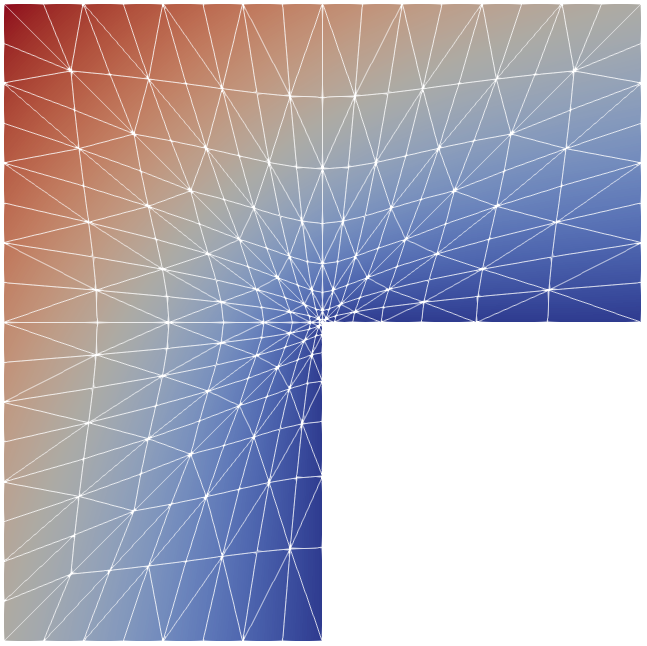
\includegraphics[width=0.35\linewidth]{Images/Test1/OT/u_OT.png}
  }
     \subfloat[\label{fig:u_OT_zoom} Zoom of the solution in the re-entrant corner.]{
    
\includegraphics[width=0.34\linewidth]{Images/Test1/OT/u_OT_zoom.png}
  }
\caption{Solution of eq.\eqref{eq:poisson_corner} on the OT mesh with $\gamma = 0.53$.}  
\label{fig:OT_mesh}
\end{figure}


\begin{figure}[h!]\label{tixz:conv_rate_summary_L}
\centering
\subfloat[\label{fig:L2_summary_L} $\leb{2}$ error]{
\begin{tikzpicture}
  \begin{axis}[
      cycle list/Dark2,
      thick,
      xmode=log,
      ymode=log,
      xlabel=$\dim \fes$,
      ylabel=$\Norm{u - u_{h}}_{\leb{2}(\W)}$,
      grid=both,
      minor grid style={gray!25},
      major grid style={gray!25},
      width=0.5\linewidth,
      %no marks,
     legend style={at={(0.0,0.0)},anchor=south west},
    ]
%\addplot+[color=yellow,mark = +]
%	table[x=dof,y=error, col sep=comma]{Data/Test1/radial/radial.csv};
%\addlegendentry{radial};
\addplot+[color=black,mark = triangle]
	table[x=dof,y=error, col sep=comma]{Data/Test1/uniform/uniform.csv};
\addlegendentry{uniform};
\addplot+[color=green, mark = diamond]
	table[x=dof,y=error, col sep=comma]{Data/Test1/h-adaptive/MS/href.csv};
\addlegendentry{h-refinement};
\addplot+[color=orange, mark = square]
	table[x=dof,y=error, col sep=comma]{Data/Test1/r-adaptive/curvature/curvature.csv};
\addlegendentry{Winslow'};
\addplot+[color=red, mark = otimes]
	table[x=dof,y=error, col sep=comma]{Data/Test1/OT/a_priori/errorL2_0.53.csv};
\addlegendentry{a-priori};
\draw[dotted] (1000,0.001) -- (1000000,0.000001);
\node at (45000,0.00001) {$1.0$};
\draw[dotted] (1000,0.004) -- (100000,0.0002);
\node at (45000,0.0008) {$0.67$};      
%\gamma = 0.53
\end{axis}
\end{tikzpicture}
}\subfloat[\label{fig:Linfty_summary_L} $\leb{\infty}$ error]{
\begin{tikzpicture}
  \begin{axis}[
      cycle list/Dark2,
      thick,
      xmode=log,
      ymode=log,
      xlabel=$\dim \fes$,
      ylabel=$\Norm{u - u_{h}}_{\leb{\infty}(\W)}$,
      grid=both,
      minor grid style={gray!25},
      major grid style={gray!25},
      width=0.5\linewidth,
      %no marks,
     legend style={at={(0.0,0.0)},anchor=south west},
    ]
\addplot+[color=black,mark = triangle]
	table[x=dof,y=error, col sep=comma]{Data/Test1/uniform/uniform_Linfty.csv};
%\addlegendentry{uniform};
\addplot+[color=green, mark = diamond]
	table[x=dof,y=error, col sep=comma]{Data/Test1/h-adaptive/MS/href_Linfty.csv};
%\addlegendentry{h-refinement};
\addplot+[color=red, mark = otimes]
	table[x=dof,y=error, col sep=comma]{Data/Test1/OT/a_priori/errorLinfty_0.67.csv};
%\addlegendentry{a-priori};
\draw[dotted,black] (100000,0.0045) -- (1000000,0.002);
\node at (500000,0.005) {$0.33$};
\draw[dotted,black] (100000,0.00005) -- (1000000,0.000005);
\node at (500000,0.000005) {$1.0$};      
\end{axis}
\end{tikzpicture}
}
\caption{Asymptotic convergence rates for different adaptive strategies in the $\leb{2}$ and  $\leb{\infty}$ norm. The OT-mesh with optimal $\gamma$-s outperform the h-adaptive strategy both in accuracy and convergence rate in the two norms.}
\end{figure}

\clearpage
\newpage


\paragraph{Link between OT mesh and a-posteriori measure}

In this section we investigate the relationship between the a-posteriori bound $\eta_{K}$ used for h-adaptivity and the OT mesh obtained by solving the one dimensional Monge-Ampère equation.

The h-refinement reduces the element mesh size by equidistributing $\eta_{K}$ over each element of the mesh.

We note that for the $\leb{2}$ norm $\eta_{K}$ is defined by integrating along facets of the domain, so the rescaled quantity $\eta_{K} / \sqrt{K}$ is supposed to act as a measure and behave similarly as the monitor function $m(r) = A + B r^{-2\gamma}$.


Concerning the pointwise $\leb{\infty}$ a-posteriori bound, the correct rescaling to define a measure does not change, as the quantity must still retain information about the properties of the two-dimensional cell for the refinement criterion.

The measure $\eta_{K} / \sqrt{K}$ has been computed from the OT mesh with $\dim \fes = 7 \times 10^{4}$ as a function of the distance from the re-entrant corner. The plots clearly show the polynomial dependence of the rescaled measures as observed for $m(r)$.
 

\begin{figure}[h!]\label{tikz:measure_OT}
\centering
\subfloat[{\label{fig:measure_OT_L2}} $\leb{2}$ norm]{
\begin{tikzpicture}
  \begin{axis}[
      cycle list/Dark2,
      thick,
      xmode=log,
      ymode = log,
      xlabel=$r$,
      ylabel=$\eta_{K}/\sqrt{|K|}$,
       xmin=1.5e-3,xmax=3e-2,
     % ymin=1e-3,
     % ymax=5e-1,
      grid=both,
      minor grid style={gray!25},
      major grid style={gray!25},
      width=0.55\linewidth,
      %no marks,
      legend style={at={(1.3,1.0)},anchor=north east},
      ]
%\draw[ultra thick,black] (0.002,0.006) -- (0.008,0.0058);  
%\draw[ultra thick,black] (0.002,0.007) -- (0.008,0.001);   
\addplot+[color=black, mark = triangle]
table[x=dist,y=measure, col sep=comma]{Data/Test1/OT/measure_L2/measure_L2_0.47.csv};
\addlegendentry{$\gamma = 0.47$}; 
\addplot+[color=red, mark = triangle]
table[x=dist,y=measure, col sep=comma]{Data/Test1/OT/measure_L2/measure_L2_0.53.csv};
\addlegendentry{$\gamma = 0.53$}; 
\addplot+[color=green, mark = triangle]
table[x=dist,y=measure, col sep=comma]{Data/Test1/OT/measure_L2/measure_L2_0.59.csv};
\addlegendentry{$\gamma = 0.59$}; 
\addplot+[color=blue, mark = triangle]
table[x=dist,y=measure, col sep=comma]{Data/Test1/OT/measure_L2/measure_L2_0.65.csv};
\addlegendentry{$\gamma = 0.65$}; 
\addplot+[color=cyan, mark = triangle]
table[x=dist,y=measure, col sep=comma]{Data/Test1/OT/measure_L2/measure_L2_0.71.csv};
\addlegendentry{$\gamma = 0.71$}; 
\addplot+[color=magenta, mark = triangle]
table[x=dist,y=measure, col sep=comma]{Data/Test1/OT/measure_L2/measure_L2_0.78.csv};
\addlegendentry{$\gamma = 0.78$}; 
\addplot+[color=orange, mark = triangle]
table[x=dist,y=measure, col sep=comma]{Data/Test1/OT/measure_L2/measure_L2_0.84.csv};
\addlegendentry{$\gamma = 0.84$}; 
\end{axis}
\end{tikzpicture}
}\\
\centering
\subfloat[{\label{fig:measure_OT_Linfty}} $\leb{\infty}$ norm]{
\begin{tikzpicture}
  \begin{axis}[
      cycle list/Dark2,
      thick,
      xmode=log,
      ymode = log,
      xlabel=$r$,
      ylabel=$\eta_{K}$,
      xmin=1e-7,xmax=2e-2,
      grid=both,
      minor grid style={gray!25},
      major grid style={gray!25},
      width=0.55\linewidth,
      legend style={at={(1.3,1.0)},anchor=north east},
    ]
    % \draw[ultra thick,black] (0.002,0.005) -- (0.008,0.00047);
\addplot+[color=black, mark = triangle]
table[x=dist,y=measure, col sep=comma]{Data/Test1/OT/measure_Linfty/measure_Linfty_0.62.csv};
\addlegendentry{$\gamma = 0.62$}; 
\addplot+[color=red, mark = triangle]
table[x=dist,y=measure, col sep=comma]{Data/Test1/OT/measure_Linfty/measure_Linfty_0.65.csv};
\addlegendentry{$\gamma = 0.65$}; 
\addplot+[color=green, mark = triangle]
table[x=dist,y=measure, col sep=comma]{Data/Test1/OT/measure_Linfty/measure_Linfty_0.67.csv};
\addlegendentry{$\gamma = 0.67$}; 
\addplot+[color=blue, mark = triangle]
table[x=dist,y=measure, col sep=comma]{Data/Test1/OT/measure_Linfty/measure_Linfty_0.71.csv};
\addlegendentry{$\gamma = 0.71$}; 
\addplot+[color=cyan, mark = triangle]
table[x=dist,y=measure, col sep=comma]{Data/Test1/OT/measure_Linfty/measure_Linfty_0.74.csv};
\addlegendentry{$\gamma = 0.74$}; 
\addplot+[color=magenta, mark = triangle]
table[x=dist,y=measure, col sep=comma]{Data/Test1/OT/measure_Linfty/measure_Linfty_0.78.csv};
\addlegendentry{$\gamma = 0.78$}; 
\addplot+[color=orange, mark = triangle]
table[x=dist,y=measure, col sep=comma]{Data/Test1/OT/measure_Linfty/measure_Linfty_0.81.csv};
\addlegendentry{$\gamma = 0.81$}; 
\end{axis}
\end{tikzpicture}
}
\caption{a-posteriori measure from OT mesh.}
\end{figure}


\clearpage
\newpage

\subsection{Crack domain}
\label{sec:Crack_domain}

Let $\W$ be the domain with a crack $ (-1,1) \times (1,1) \slash ([0,1) \times {0}])$. The solution of Equation \ref{eq:poisson_corner} is 

\begin{equation}
    u(r,\theta) = r^{1/2} sin(\theta/2)
\label{eq:exact_solution_crack}
\end{equation}

Numerically, $\omega$ has been set to $2\pi - \epsilon$ with $\epsilon = 10^{-3}$.

\begin{figure}[h!]
\centering
\subfloat[{\label{fig:crack_h_ref-0.0}} Mesh obtained with h-refinement ($\beta = 0.0$)]{
    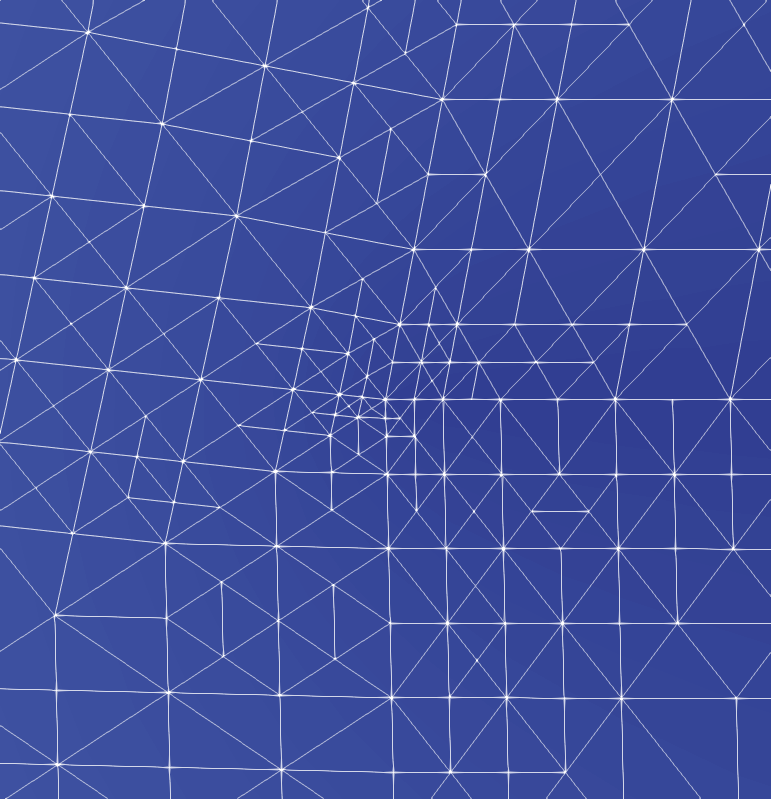
\includegraphics[scale=0.18]{Images/Test2/h-adaptive/u_0.0.png}
  }
\subfloat[{\label{fig:crack_h_ref-0.99}} Mesh obtained with h-refinement ($\beta = 0.99$)]{
    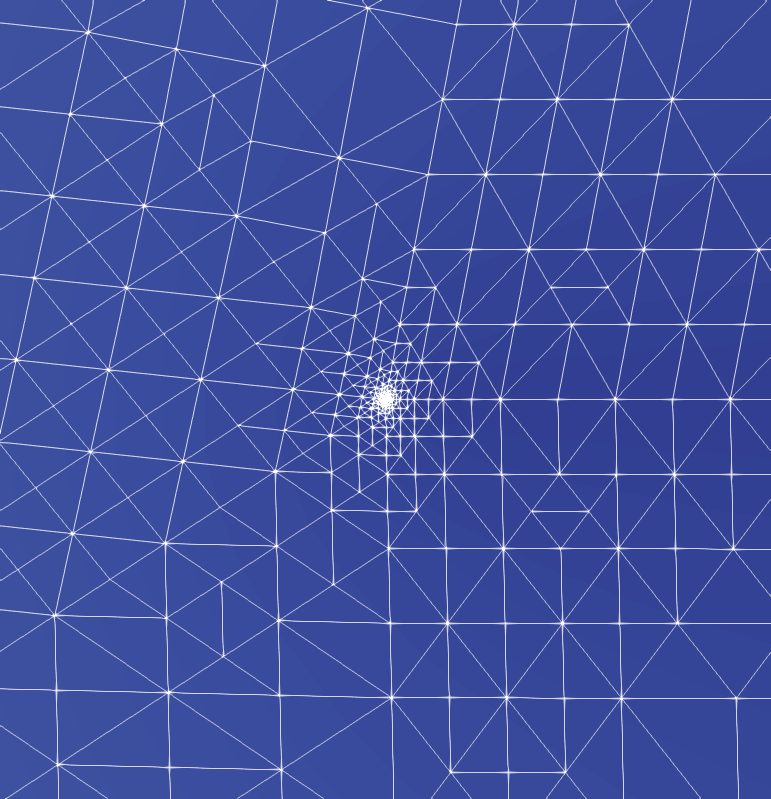
\includegraphics[scale=0.18]{Images/Test2/h-adaptive/u_0.99.png}
  }\\
\centering
\subfloat[{\label{fig:Winslow posteriori}} Mesh obtained with Winslow' method]{
    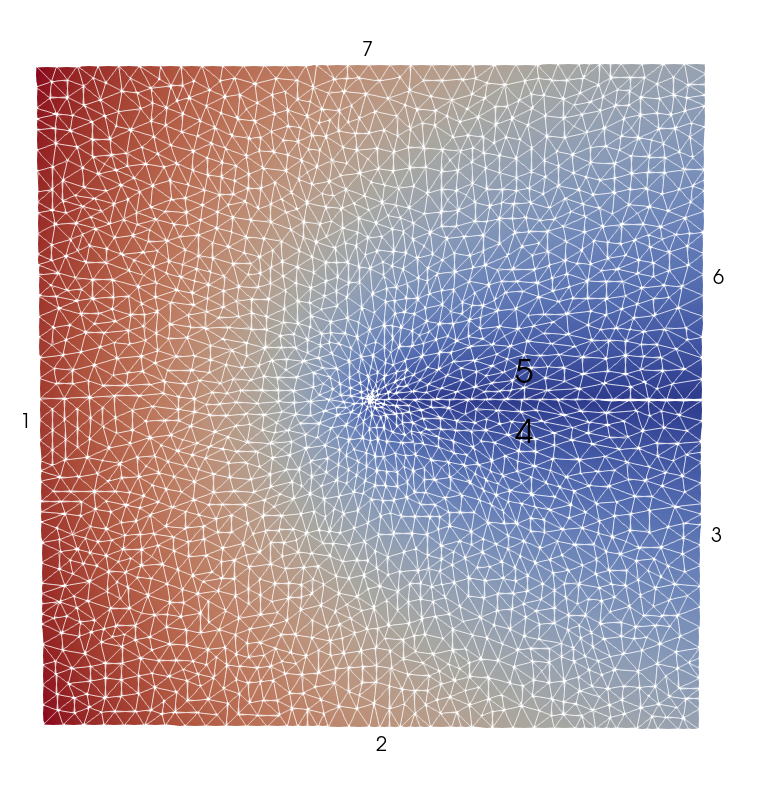
\includegraphics[scale=0.23]{Images/Test2/r-adaptive/u_0.99_11862.png}
}
\subfloat[{\label{fig:Winslow_computational_domain}}
    Computational domain for Winslow's method ]{
    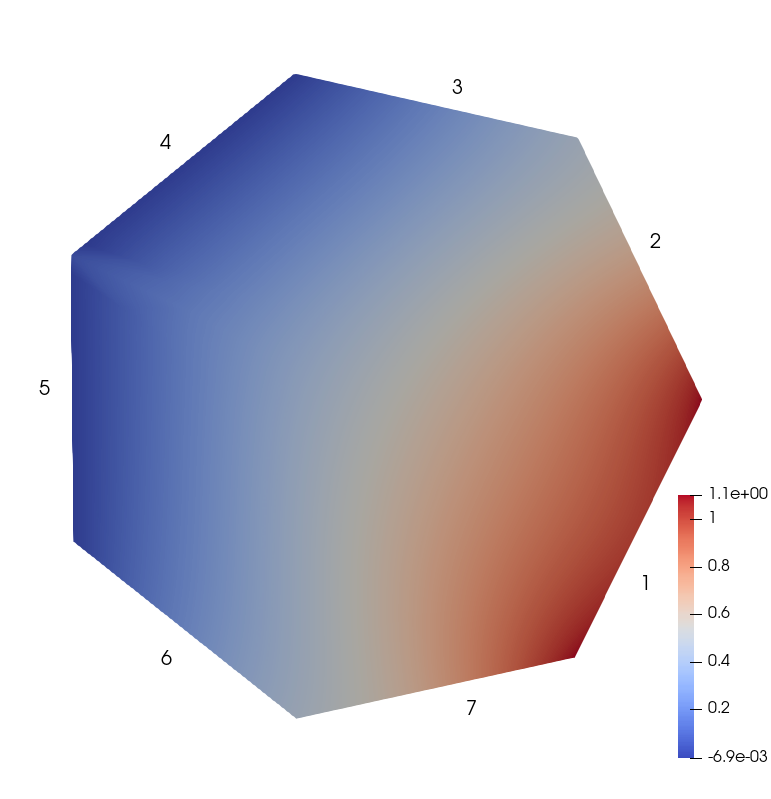
\includegraphics[scale=0.23]{Images/Test2/r-adaptive/u_c.png}
  }\\
\centering
\subfloat[{\label{fig:crack_OT}}
    OT mesh
  ]{
    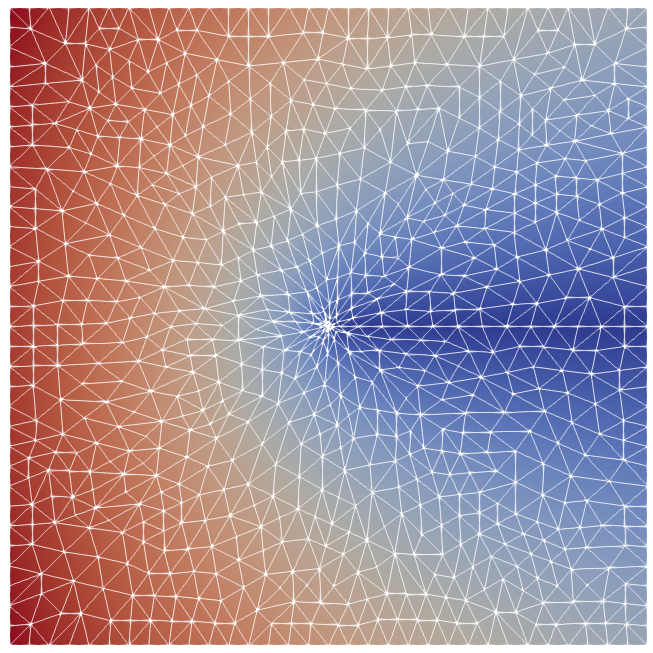
\includegraphics[scale=0.23]{Images/Test2/OT/u_OT.png}
}
\subfloat[{\label{fig:crack_OT_zoom}}
    Zoom of OT mesh near the corner
  ]{
    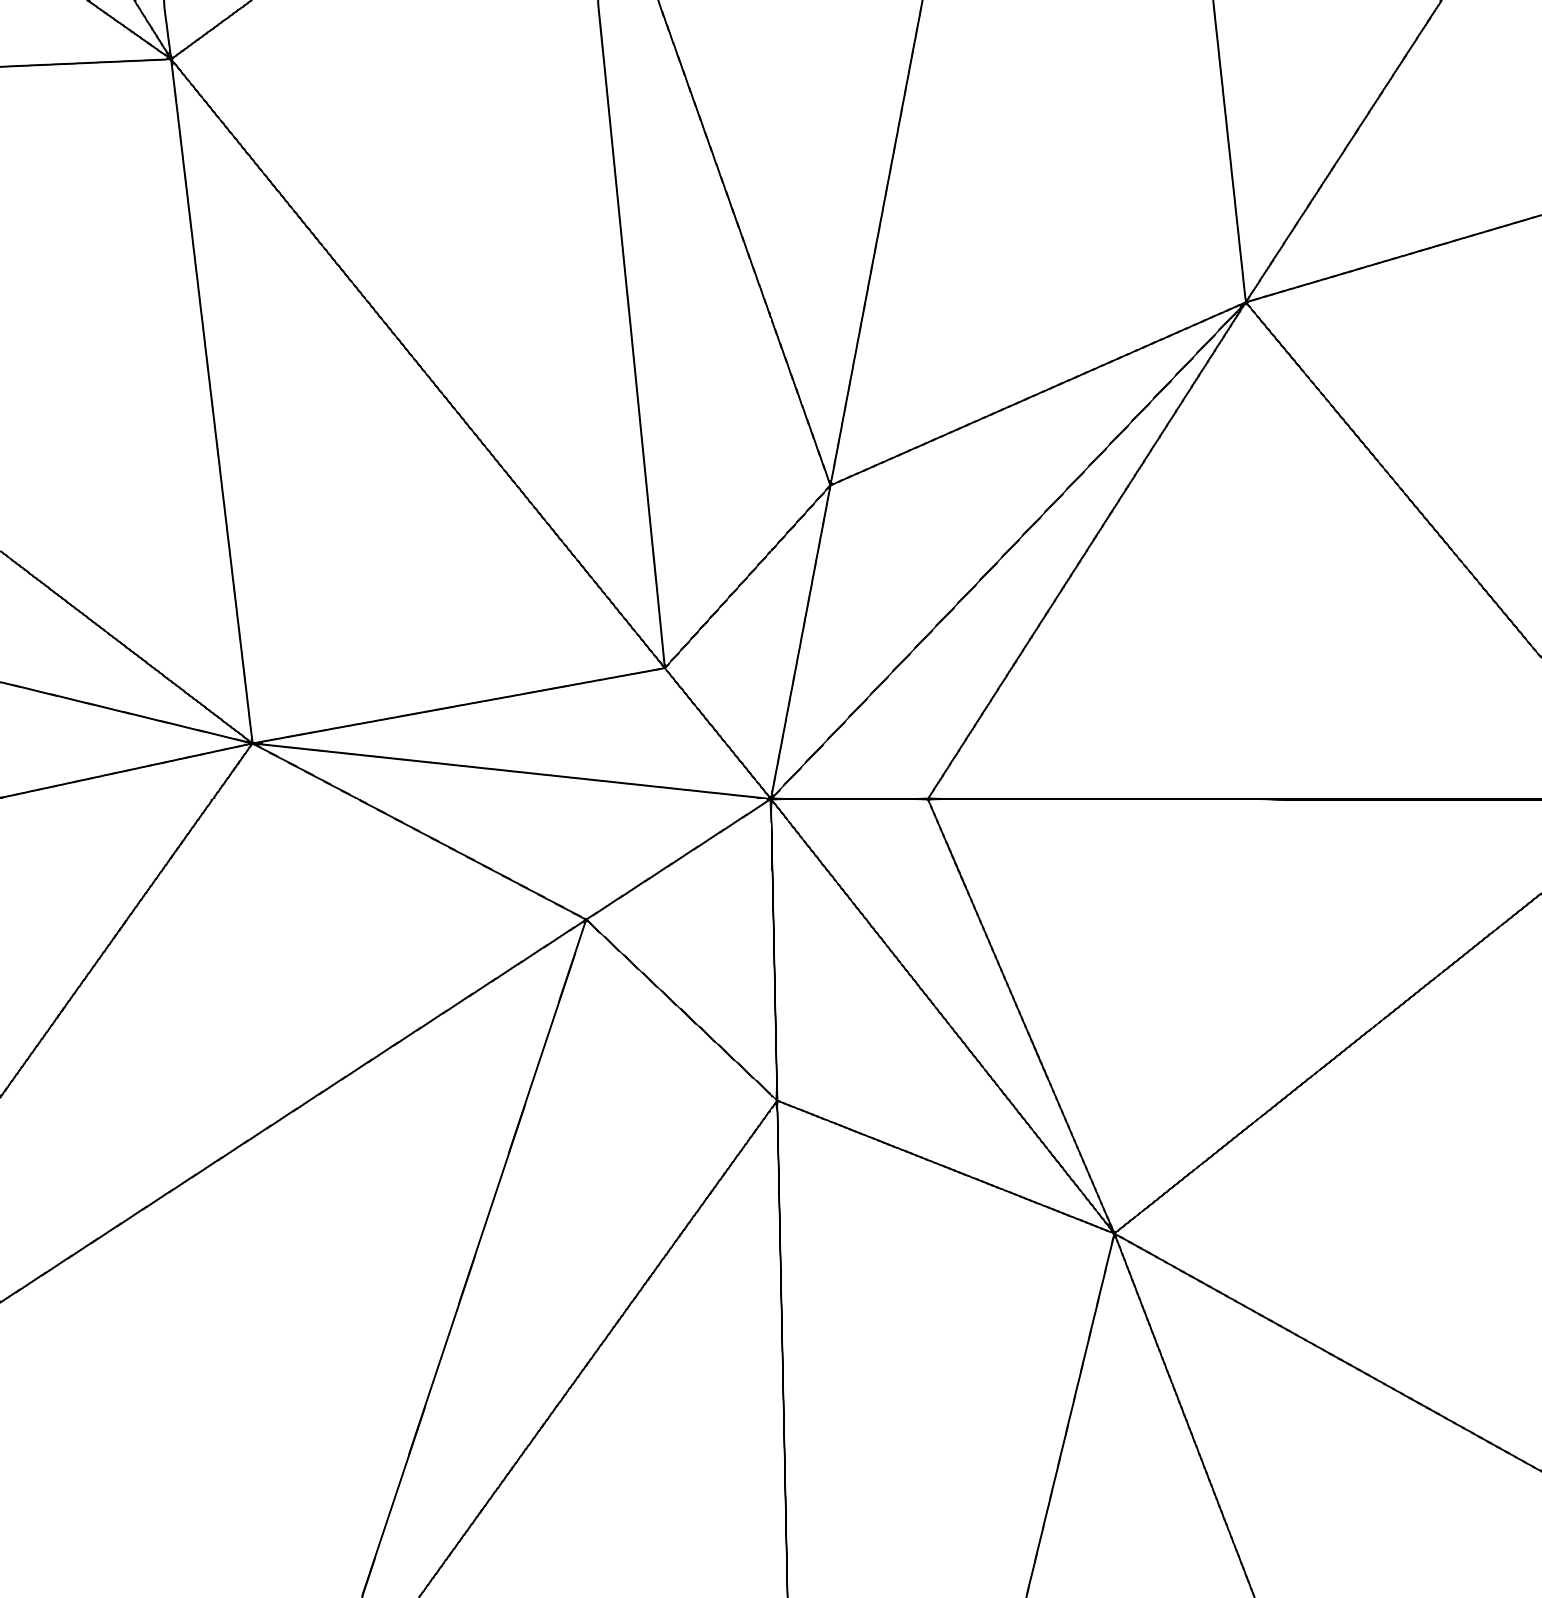
\includegraphics[scale=0.185]{Images/Test2/OT/u_OT_zoom.png}
  }
\end{figure}

\clearpage
\newpage


\paragraph{OT mesh for different $\gamma$}

In this Section, we show how the parameter $\gamma$ affects the accuracy and the quality of the resulting OT mesh. 


\begin{figure}[h!]%\label{tikz:OT_gamma_error_crack}
\centering
\subfloat[{\label{fig:crack_error_L2}} $\leb{2}$ error for different $\gamma$]{  
\begin{tikzpicture}
  \begin{axis}[
      cycle list/Dark2,
      thick,
      xmode=log,
      ymode=log,
      xlabel=$\dim \fes$,
      ylabel=$\Norm{u - u_{h}}_{\leb{2}(\W)}$,
      grid=both,
      minor grid style={gray!25},
      major grid style={gray!25},
      width=0.5\linewidth,
      %no marks,
      legend style={at={(0.0,0.0)},anchor=south west},
    ]
\addplot+[color=black,mark = triangle]
        table[x=dof,y=error, col sep=comma]{Data/Test2/OT/a_priori/errorL2_0.0.csv};
\addlegendentry{$\gamma = 0.0$};
\addplot+[color=red,mark = triangle]
	table[x=dof,y=error, col sep=comma]{Data/Test2/OT/a_priori/errorL2_0.2.csv};
\addlegendentry{$\gamma = 0.2$};
%\addplot+[color=green,mark = triangle]
%	table[x=dof,y=error, col sep=comma]{Data/Test2/OT/a_priori/errorL2_0.33.csv};
%\addlegendentry{$\gamma = 0.33$};        
\addplot+[color=green,mark = triangle]
	table[x=dof,y=error, col sep=comma]{Data/Test2/OT/a_priori/errorL2_0.5.csv};
\addlegendentry{$\gamma = 0.5$};
\addplot+[color=blue,mark = triangle]
	table[x=dof,y=error, col sep=comma]{Data/Test2/OT/a_priori/errorL2_0.6.csv};
\addlegendentry{$\gamma = 0.6$};        
\addplot+[color=cyan,mark = triangle]
	table[x=dof,y=error, col sep=comma]{Data/Test2/OT/a_priori/errorL2_0.75.csv};
\addlegendentry{$\gamma = 0.75$};
\addplot+[color=magenta,mark = triangle]
        table[x=dof,y=error,col sep=comma]{Data/Test2/OT/a_priori/errorL2_0.8.csv};
\addlegendentry{$\gamma = 0.8$};
\addplot+[color=yellow,mark = triangle]
	table[x=dof,y=error, col sep=comma]{Data/Test2/OT/a_priori/errorL2_0.9.csv};
\addlegendentry{$\gamma = 0.9$};        
\end{axis}
\end{tikzpicture}
}
\subfloat[{\label{fig:crack_error_Linfty}} $\leb{\infty}$ error for different $\gamma$]{  
\begin{tikzpicture}
  \begin{axis}[
      cycle list/Dark2,
      thick,
      xmode=log,
      ymode=log,
      xlabel=$\dim \fes$,
      ylabel=$\Norm{u - u_{h}}_{\leb{\infty}(\W)}$,
      grid=both,
      minor grid style={gray!25},
      major grid style={gray!25},
      width=0.5\linewidth,
      %no marks,
      %legend style={at={(0.0,0.0)},anchor=south west},
    ]
\addplot+[color=black,mark = triangle]
        table[x=dof,y=error, col sep=comma]{Data/Test2/OT/a_priori/errorLinfty_0.0.csv};
%\addlegendentry{$\gamma = 0.0$};
\addplot+[color=red,mark = triangle]
	table[x=dof,y=error, col sep=comma]{Data/Test2/OT/a_priori/errorLinfty_0.2.csv};
%\addlegendentry{$\gamma = 0.2$};
\addplot+[color=green,mark = triangle]
	table[x=dof,y=error, col sep=comma]{Data/Test2/OT/a_priori/errorLinfty_0.33.csv};
%\addlegendentry{$\gamma = 0.33$};        
\addplot+[color=green,mark = triangle]
	table[x=dof,y=error, col sep=comma]{Data/Test2/OT/a_priori/errorLinfty_0.5.csv};
%\addlegendentry{$\gamma = 0.5$};
\addplot+[color=blue,mark = triangle]
	table[x=dof,y=error, col sep=comma]{Data/Test2/OT/a_priori/errorLinfty_0.6.csv};
%\addlegendentry{$\gamma = 0.6$};
\addplot+[color=cyan,mark = triangle]
	table[x=dof,y=error, col sep=comma]{Data/Test2/OT/a_priori/errorLinfty_0.75.csv};
%\addlegendentry{$\gamma = 0.75$};
\addplot+[color=magenta,mark = triangle]
        table[x=dof,y=error, col sep=comma]{Data/Test2/OT/a_priori/errorLinfty_0.8.csv};
%\addlegendentry{$\gamma = 0.8$};
\addplot+[color=yellow,mark = triangle]
	table[x=dof,y=error, col sep=comma]{Data/Test2/OT/a_priori/errorLinfty_0.9.csv};
%\addlegendentry{$\gamma = 0.9$};        
\end{axis}
\end{tikzpicture}
}\\
\subfloat[{\label{fig:q_gamma}} mesh condition of OT mesh for different $\gamma$]{  
\begin{tikzpicture}
  \begin{axis}[
      cycle list/Dark2,
      thick,
      xmode=log,
      ymode=log,
      xlabel=$\dim \fes$,
      ylabel=$q$,
      grid=both,
      minor grid style={gray!25},
      major grid style={gray!25},
      width=0.5\linewidth,
      %no marks,
      %legend style={at={(0.1,0.1)},anchor=south west},
    ]
%\addplot+[color=black,mark = triangle]
%        table[x=dof,y=q, col sep=comma]{Data/Test1/OT/a_priori/stat_0.0.csv};
%\addlegendentry{$\gamma = 0.0$};
\addplot+[color=red,mark = triangle]
	table[x=dof,y=q, col sep=comma]{Data/Test2/OT/a_priori/stat_0.2.csv};
%\addlegendentry{$\gamma = 0.2$};
%\addplot+[color=green,mark = triangle]
%	table[x=dof,y=q, col sep=comma]{Data/Test2/OT/a_priori/stat_0.33.csv};
%\addlegendentry{$\gamma = 0.33$};        
\addplot+[color=green,mark = triangle]
      table[x=dof,y=q, col sep=comma]{Data/Test2/OT/a_priori/stat_0.5.csv};
%\addlegendentry{$\gamma = 0.5$};
\addplot+[color=blue,mark = triangle]
	table[x=dof,y=q, col sep=comma]{Data/Test2/OT/a_priori/stat_0.6.csv};
%\addlegendentry{$\gamma = 0.6$};  
\addplot+[color=cyan,mark = triangle]
	table[x=dof,y=q, col sep=comma]{Data/Test2/OT/a_priori/stat_0.75.csv};
%\addlegendentry{$\gamma = 0.75$};
\addplot+[color=magenta,mark = triangle]
        table[x=dof,y=q, col sep=comma]{Data/Test2/OT/a_priori/stat_0.8.csv};
%\addlegendentry{$\gamma = 0.8$};
\addplot+[color=yellow,mark = triangle]
	table[x=dof,y=q, col sep=comma]{Data/Test2/OT/a_priori/stat_0.9.csv};
%\addlegendentry{$\gamma = 0.9$};        
\end{axis}
\end{tikzpicture}
}\subfloat[{\label{fig:mu_gamma}} shape regularity for different $\gamma$]{  
\begin{tikzpicture}
  \begin{axis}[
      cycle list/Dark2,
      thick,
      xmode=log,
      ymode=log,
      xlabel=$\dim \fes$,
      ylabel=$\mu$,
      grid=both,
      minor grid style={gray!25},
      major grid style={gray!25},
      width=0.5\linewidth,
      %no marks,
      %legend style={at={(0.1,0.1)},anchor=south west},
    ]
%\addplot+[color=black,mark = triangle]
%        table[x=dof,y=mu, col sep=comma]{Data/Test1/OT/a_priori/stat_0.0.csv};
%\addlegendentry{$\gamma = 0.0$};
\addplot+[color=red,mark = triangle]
	table[x=dof,y=mu, col sep=comma]{Data/Test2/OT/a_priori/stat_0.2.csv};
%\addlegendentry{$\gamma = 0.2$};
%\addplot+[color=green,mark = triangle]
%	table[x=dof,y=mu, col sep=comma]{Data/Test2/OT/a_priori/stat_0.33.csv};
%\addlegendentry{$\gamma = 0.33$};        
\addplot+[color=green,mark = triangle]
	table[x=dof,y=mu, col sep=comma]{Data/Test2/OT/a_priori/stat_0.5.csv};
%\addlegendentry{$\gamma = 0.5$};
\addplot+[color=blue,mark = triangle]
	table[x=dof,y=mu, col sep=comma]{Data/Test2/OT/a_priori/stat_0.6.csv};
%\addlegendentry{$\gamma = 0.6$};
\addplot+[color=cyan,mark = triangle]
	table[x=dof,y=mu, col sep=comma]{Data/Test2/OT/a_priori/stat_0.75.csv};
%\addlegendentry{$\gamma = 0.75$};
\addplot+[color=magenta,mark = triangle]
        table[x=dof,y=mu, col sep=comma]{Data/Test2/OT/a_priori/stat_0.8.csv};
%\addlegendentry{$\gamma = 0.8$};
\addplot+[color=yellow,mark = triangle]
	table[x=dof,y=mu, col sep=comma]{Data/Test2/OT/a_priori/stat_0.9.csv};
%\addlegendentry{$\gamma = 0.9$};        
\end{axis}
\end{tikzpicture}
}
\caption{error and quality measure for OT mesh for different $\gamma$}
\end{figure}



\begin{figure}
\centering
\subfloat[{\label{fig:L2_gamma}} Error as function of $\gamma$]{  
\begin{tikzpicture}
  \begin{axis}[
      cycle list/Dark2,
      thick,
      xmode=log,
      ymode=log,
      xlabel=$\gamma$,
      ylabel=$Error$,
      grid=both,
      minor grid style={gray!25},
      major grid style={gray!25},
      width=0.5\linewidth,
      %no marks,
      %legend style={at={(0.1,0.1)},anchor=south west},
    ]
\addplot+[color=red,mark = triangle]
	table[x=gamma,y=error_L2, col sep=comma]{Data/Test2/OT/a_priori/error_gamma.csv};
\addlegendentry{$\leb{2}$ error};
\addplot+[color=green,mark = triangle]
	table[x=gamma,y=error_Linfty, col sep=comma]{Data/Test2/OT/a_priori/error_gamma.csv};
\addlegendentry{$\leb{\infty}$ error};               
\end{axis}
\end{tikzpicture}
}\\
\subfloat[{\label{fig:mu_gamma2}} Shape regularity]{  
\begin{tikzpicture}
  \begin{axis}[
      cycle list/Dark2,
      thick,
      xmode=log,
      ymode=log,
      xlabel=$\gamma$,
      ylabel=$\mu$,
      grid=both,
      minor grid style={gray!25},
      major grid style={gray!25},
      width=0.35\linewidth,
      %no marks,
      %legend style={at={(0.1,0.1)},anchor=south west},
    ]
\addplot+[color=red,mark = triangle]
table[x=gamma,y=mu, col sep=comma]{Data/Test2/OT/a_priori/stat_gamma.csv};
\end{axis}
\end{tikzpicture}
}
\subfloat[{\label{fig:q_gamma2}} Mesh condition]{  
\begin{tikzpicture}
  \begin{axis}[
      cycle list/Dark2,
      thick,
      xmode=log,
      ymode=log,
      xlabel=$\gamma$,
      ylabel=$q$,
      grid=both,
      minor grid style={gray!25},
      major grid style={gray!25},
      width=0.35\linewidth,
      %no marks,
      %legend style={at={(0.1,0.1)},anchor=south west},
    ]
\addplot+[color=red,mark = triangle]
table[x=gamma,y=q, col sep=comma]{Data/Test2/OT/a_priori/stat_gamma.csv};
\end{axis}
\end{tikzpicture}
}
\caption{Error and quality measures for the a-priori OT mesh as function of $\gamma$ with dof = 74880.}
\end{figure}


\begin{figure}[h!]\label{tikz:h-ref}
\centering
\subfloat[\label{L2_norm_summary_crack} $\leb{2}$ norm]{  
\begin{tikzpicture}
  \begin{axis}[
      cycle list/Dark2,
      thick,
      xmode=log,
      ymode=log,
      xlabel=$\dim \fes$,
      ylabel=$\Norm{u - u_{h}}_{\leb{2}(\W)}$,
      grid=both,
      minor grid style={gray!25},
      major grid style={gray!25},
      width=0.5\linewidth,
      %no marks,
      legend style={at={(0.0,0.0)},anchor=south west},
    ]
\addplot+[color=black,mark = triangle]
	table[x=dof,y=error, col sep=comma]{Data/Test2/uniform/uniform.csv};
\addlegendentry{unstructured};
\addplot+[color=green, mark = star]
	table[x=dof,y=error, col sep=comma]{Data/Test2/h-adaptive/href_0.99.csv};
\addlegendentry{h-ref ($\beta: $ 0.99)};
\addplot+[color=red, mark = diamond]
table[x=dof,y=error, col sep=comma]{Data/Test2/OT/a_priori/errorL2_0.6.csv};
\addlegendentry{OT a-priori};
%\gamma = 0.6
\addplot+[color=orange, mark = square]
	table[x=dof,y=error, col sep=comma]{Data/Test2/r-adaptive/a-posteriori/beta_0.99/posteriori.csv};
\addlegendentry{Winslow'};
\draw[dotted,black] (100000,0.0007) -- (300000,0.0004);
\node at (140000,0.001) {$0.5$};
\draw[dotted,black] (100000,0.00006) -- (1000000,0.000008);
\node at (140000,0.000013) {$1.0$};
\end{axis}
\end{tikzpicture}
}
\subfloat[\label{Linfty_norm_summary_crack} $\leb{\infty}$ norm]{  
\begin{tikzpicture}
  \begin{axis}[
      cycle list/Dark2,
      thick,
      xmode=log,
      ymode=log,
      xlabel=$\dim \fes$,
      ylabel=$\Norm{u - u_{h}}_{\leb{\infty}(\W)}$,
      grid=both,
      minor grid style={gray!25},
      major grid style={gray!25},
      width=0.5\linewidth,
      %no marks,
      legend style={at={(0.0,0.0)},anchor=south west},
    ]
\addplot+[color=black,mark = triangle]
	table[x=dof,y=error, col sep=comma]{Data/Test2/uniform/uniform_Linfty.csv};
%\addlegendentry{unstructured};
\addplot+[color=green, mark = star]
	table[x=dof,y=error, col sep=comma]{Data/Test2/h-adaptive/href_Linfty.csv};
%\addlegendentry{h-ref ($\beta: $ 0.0)};
\addplot+[color=red, mark = diamond]
table[x=dof,y=error, col sep=comma]{Data/Test2/OT/a_priori/errorL2_0.75.csv};
%\addlegendentry{OT a-priori};
\draw[dotted,black] (100000,0.045) -- (1000000,0.03);
\node at (500000,0.05) {$0.25$};
\draw[dotted,black] (100000,0.0001) -- (1000000,0.00001);
\node at (500000,0.000009) {$1.0$};    
\end{axis}
\end{tikzpicture}
}
\caption{Asymptotic convergence rates for different adaptive strategies. Note that the rate of convergence is optimal for h-refinement and the OT strategy ($\gamma = 0.7$) in both norms.}
\end{figure}

\clearpage
\newpage


\paragraph{Link between OT mesh and a-posteriori measure}

In this section we investigate the relationship between the a-posteriori bound $\eta_{K}$  and the OT mesh as we did for the L-shaped domain. The plots evidence again a polynomial dependence of the rescaled measures, as observed for $m(r)$.

\begin{figure}[h!]\label{tikz:measure_OT_crack}
\centering
\subfloat[{\label{fig:measure_OT_L2_crack}} $\leb{2}$ norm]{
\begin{tikzpicture}
  \begin{axis}[
      cycle list/Dark2,
      thick,
      xmode=log,
      ymode = log,
      xlabel=$r$,
      ylabel=$\eta_{K}/\sqrt{|K|}$,
      xmin=1e-3,xmax=3e-2,
      grid=both,
      minor grid style={gray!25},
      major grid style={gray!25},
      width=0.55\linewidth,
      %no marks,
      legend style={at={(1.3,1.0)},anchor=north east},
      ]
%\draw[ultra thick,black] (0.002,0.006) -- (0.008,0.0058);  
%\draw[ultra thick,black] (0.002,0.007) -- (0.008,0.001);   
\addplot+[color=black, mark = triangle]
table[x=dist,y=measure, col sep=comma]{Data/Test2/OT/measure_L2/measure_L2_0.47.csv};
\addlegendentry{$\gamma = 0.47$}; 
\addplot+[color=red, mark = triangle]
table[x=dist,y=measure, col sep=comma]{Data/Test2/OT/measure_L2/measure_L2_0.53.csv};
\addlegendentry{$\gamma = 0.53$}; 
\addplot+[color=green, mark = triangle]
table[x=dist,y=measure, col sep=comma]{Data/Test2/OT/measure_L2/measure_L2_0.59.csv};
\addlegendentry{$\gamma = 0.59$}; 
\addplot+[color=blue, mark = triangle]
table[x=dist,y=measure, col sep=comma]{Data/Test2/OT/measure_L2/measure_L2_0.65.csv};
\addlegendentry{$\gamma = 0.65$}; 
\addplot+[color=cyan, mark = triangle]
table[x=dist,y=measure, col sep=comma]{Data/Test2/OT/measure_L2/measure_L2_0.71.csv};
\addlegendentry{$\gamma = 0.71$}; 
\addplot+[color=magenta, mark = triangle]
table[x=dist,y=measure, col sep=comma]{Data/Test2/OT/measure_L2/measure_L2_0.78.csv};
\addlegendentry{$\gamma = 0.78$}; 
\addplot+[color=orange, mark = triangle]
table[x=dist,y=measure, col sep=comma]{Data/Test2/OT/measure_L2/measure_L2_0.84.csv};
\addlegendentry{$\gamma = 0.84$}; 
\end{axis}
\end{tikzpicture}
}\\
\centering
\subfloat[{\label{fig:measure_OT_Linfty_crack}} $\leb{\infty}$ norm]{
\begin{tikzpicture}
  \begin{axis}[
      cycle list/Dark2,
      thick,
      xmode=log,
      ymode = log,
      xlabel=$r$,
      ylabel=$\eta_{K}$,
      xmin=1e-7,xmax=1e-3,
      grid=both,
      minor grid style={gray!25},
      major grid style={gray!25},
      width=0.55\linewidth,
      %no marks,
      legend style={at={(1.3,1.0)},anchor=north east},
    ]
    % \draw[ultra thick,black] (0.002,0.005) -- (0.008,0.00047);
\addplot+[color=black, mark = triangle]
table[x=dist,y=measure, col sep=comma]{Data/Test2/OT/measure_Linfty/measure_Linfty_0.62.csv};
\addlegendentry{$\gamma = 0.62$}; 
\addplot+[color=red, mark = triangle]
table[x=dist,y=measure, col sep=comma]{Data/Test2/OT/measure_Linfty/measure_Linfty_0.65.csv};
\addlegendentry{$\gamma = 0.65$}; 
\addplot+[color=green, mark = triangle]
table[x=dist,y=measure, col sep=comma]{Data/Test2/OT/measure_Linfty/measure_Linfty_0.68.csv};
\addlegendentry{$\gamma = 0.68$}; 
\addplot+[color=blue, mark = triangle]
table[x=dist,y=measure, col sep=comma]{Data/Test2/OT/measure_Linfty/measure_Linfty_0.71.csv};
\addlegendentry{$\gamma = 0.71$}; 
\addplot+[color=cyan, mark = triangle]
table[x=dist,y=measure, col sep=comma]{Data/Test2/OT/measure_Linfty/measure_Linfty_0.74.csv};
\addlegendentry{$\gamma = 0.75$}; 
\addplot+[color=magenta, mark = triangle]
table[x=dist,y=measure, col sep=comma]{Data/Test2/OT/measure_Linfty/measure_Linfty_0.81.csv};
\addlegendentry{$\gamma = 0.81$}; 
\addplot+[color=orange, mark = triangle]
table[x=dist,y=measure, col sep=comma]{Data/Test2/OT/measure_Linfty/measure_Linfty_0.84.csv};
\addlegendentry{$\gamma = 0.84$}; 
\end{axis}
\end{tikzpicture}
}
\caption{a-posteriori measure from OT mesh.}
\end{figure}




\clearpage
\newpage

\section{Mesh Skewness}
\label{sec:skewness}
The quality of the output mesh can be expressed in terms of different measures. Besides the shape regularity, another common metric used in the context of r-adaptive methods is the \textit{skewness}, which indicates
how far mesh elements are from being equilateral. A general indicator for triangular elements has been proposed in \cite{BHR:2009} and employs the local map $Q_{K}: \widehat{K}
\rightarrow K$, with $\widehat{K} \in \T{}_{c}$ and $K \in
\T{}$. Given the corresponding Jacobian $\pmb{J}_{K}$ with eigenvalues
$\lambda_{1}$ and $\lambda_{2}$, the quality measure for the element
$K$ is defined as
\begin{equation}
  Q_{K}
  =
  \frac{1}{2} \left( \frac{\lambda_{1}}{\lambda_{2}}
  +
  \frac{\lambda_{2}}{\lambda_{1}}  \right).
  \label{eq:local skewness}
\end{equation}
We define the \emph{global quality measure} as
\begin{equation}
  Q = \max_{K \in \T{}}
  Q_{K}
\end{equation}

Under the OT transformation $\vec x = \frac{r}{s} \vec \xi$ we can determine the value of Q analytically. As the mesh gets more uniform away from the corner, we assume that $Q$ is given for cells where $r \sim 0$, so that the algebraic expression \eqref{eq:mesh_transformation} simplifies to $r^{1-\gamma} = s$. We then compute the Jacobian of the map $\vec x = s^{\frac{\gamma}{1-\gamma}} \vec \xi $:


\begin{equation*} 
 \pmb{J} =  \begin{bmatrix}
x_{\xi} & x_{\eta} \\
y_{\xi} & y_{\eta}  
\end{bmatrix} =  
\frac{\gamma}{1-\gamma} (\xi^{2} + \eta^{2})^{\frac{\gamma}{2(1-\gamma)}-1} \begin{bmatrix}
 \xi^{2} + (\xi^{2} + \eta^{2})\frac{1-\gamma}{\gamma} &  \xi \eta  \\
 \xi \eta &  \eta^{2} + (\xi^{2} + \eta^{2})\frac{1-\gamma}{\gamma}.    
\end{bmatrix}
\end{equation*}

The eigenvalues are $\lambda_{1} = \frac{1-\gamma}{\gamma}(\xi + \nu)^{2}$ and $\lambda_{2} = \frac{1}{\gamma}(\xi + \nu)^{2}$. Finally, the skewness is expressed in terms of the interior angle $\omega$ by:

\begin{equation}
 Q(\omega) = \frac{1}{2}\left(\frac{\lambda_{1}}{\lambda_{2}} + \frac{\lambda_{2}}{\lambda_{1}}\right) =  \frac{1}{2}\left((1-\gamma) + \frac{1}{(1-\gamma)}\right) =  \frac{1}{2}\left(\left(\frac{\pi}{2\omega}\right) + \left(\frac{2\omega}{\pi}\right)\right).
\end{equation}

We can further simplify the expression by writing $\omega = t\pi$, with $1 < t < 2$:

\begin{equation}
 Q(t) = \frac{1 + 4t^{2}}{4t}, \quad t \in (1,2).
\end{equation}

This shows that the mesh quality is supposed to deteriorate as the interior angle increases.


\begin{figure}[h!]\label{tikz:comparison-rate}
\centering
\begin{tikzpicture}
  \begin{axis}[
      cycle list/Dark2,
      thick,
      xmode=log,
      ymode = log,
      xlabel=$\dim \fes$,
      ylabel=$Q$,
      grid=both,
      minor grid style={gray!25},
      major grid style={gray!25},
      width=0.4\linewidth,
      %no marks,
      %legend style={at={(0.1,0.1)},anchor=south west},
    ]

\addplot+[color=red, mark = triangle]
	table[x=dof,y=Q, col sep=comma]{Data/Test1/OT/skewness_L.csv};
\addlegendentry{$\omega = \frac{3}{2} \pi$};
\addplot+[color=red, mark = star,dotted]
	table[x=dof,y=Q_theory, col sep=comma]{Data/Test1/OT/skewness_L.csv};
\addlegendentry{};
\addplot+[color=cyan, mark = triangle]
	table[x=dof,y=Q, col sep=comma]{Data/Test2/OT/skewness_crack.csv};
\addlegendentry{$\omega = 2 \pi$};
\addplot+[color=cyan, mark = star,dotted]
table[x=dof,y=Q_theory, col sep=comma]{Data/Test2/OT/skewness_crack.csv};
\addlegendentry{};
\end{axis}
\end{tikzpicture}
\caption{Mesh skewness for L-shaped domain $(\omega = \frac{3}{2}\pi)$ and crack domain $(\omega = 2\pi)$}
\end{figure}


\clearpage
\newpage

\section{Conclusions}
\label{sec:conclusion}

In this paper, we have analysed different adaptive mesh methods for the solution of the Poisson equation on two non-convex domains. We first derived its SIP-dG variational form using the theoretical framework of the weighted Sobolev spaces. We stated the Theorem of existence and uniqueness of the solution, provided that a weight $\beta$ is greater than a specif threshold, based on the geometry of the non-convex domain. 

Our first contribution consisted in the derivation of an \textit{a-posteriori} error upper bound for the SIP-dG method in the $\leb{2}$ norm. This has enabled us to obtain a local error estimator that drives the mesh adaptation for various $h$- and $r$-adaptive strategies. 

The ms $h$-refinement has showed optimal order of convergence independently on the parameter $\hat{\beta}$. This suggests that $\hat{\beta}$ does not directly affect $\beta_{min}$, required for the existence of the solution of the Poisson equation.

Concerning the moving mesh methods, we first conducted numerical tests using the \textit{Winslow's} MMPDE for three different monitor functions. We observed that the a-posteriori monitor function outperforms that ones given by the gradient and curvature of the numerical solution. This should encourage the research community involved in moving mesh methods to adopt a model-dependent monitor function, provided that an a-posteriori indicator is available. 

An \textit{Optimal Transport} mesh has also been devised, inspired by the strong dependence of the solution on the radial variable near the re-entrant corner. This method is more accurate than Winslow's strategy. Furthermore, the computational cost is much cheaper as does not require the numerical solution of a PDE with a semi-implicit time discretisation. Concerning the mesh quality, we computed the \textit{mesh skewness} analytically, which proves that as the interior angle increases the mesh quality deteriorates. 


Finally, we have compared the quality of all the adaptive meshes in terms of \textit{mesh condition} and \textit{shape regularity}. With regard to the L-shaped domain, the h-refinement strategy achieves lowest mesh condition and highest shape regularity. Concerning the crack domain, the shape regularity of OT mesh decreases, as suggested by the \textit{skewness} metric in \S \ref{sec:skewness}, but is independent on the dimension of the Galerkin space. On the contrary, the quality of the Winslow's mesh decreases dramatically, resulting in a very skewed mesh for high degrees of freedom.

In conclusion, we have established that the a-posteriori estimator provides optimal order of convergence for both $h$- and some $r$-refinement strategies. The Winslow's method is not reliable as the resulting mesh becomes too skewed for increasing dofs, while the quality of the OT mesh is independent on the dimension of the Galerkin space and its accuracy is comparable to that one of h-refinement.\\

In the view of the above considerations, our future research directions on this topic will examine:

\begin{enumerate}
\item Thorough investigation on the dependence of the a-posteriori estimator with respect to the weight $\beta$, which defines the weighted Sobolev space;
\item Scalability of the algorithms through parallelisation;
\item Extension of the OT strategy by solving a Monge-Ampère type equation \cite{BRW:2015}; 
\item The application of the $h$-refinement and OT strategy to other relevant time-dependent problems arising in physics, such as the Shallow-Water equations in non-convex domains.
\end{enumerate}


\clearpage
\newpage

\appendix


\section{Derivation of optimal $\gamma$ for \leb{\infty} and \leb{2} norm}

\subsection{\leb{\infty} norm}

We derive here the optimal value of the exponent $\gamma$ that minimises the $\leb{\infty}$ norm. We consider the function $u(r) = r^{\alpha}$, where $\alpha$ is a parameter that depends on the interior angle of the re-entrant corner. 
As $\alpha < 1$ and $u \not\in C^{2}[0,1]$, we must split the error analysis into two parts. Then, we write 

$$\Norm{u - p_{1,N}}_{\infty,[0,1]} = \max \{ \Norm{u - p_{1,N}}_{\infty,[0,x_{1}]}, \Norm{u - p_{1,N}}_{\infty,[x_{1},1]}\}$$

For the first part, by triangle inequality

\begin{equation}
\label{eq:ineq1}
\Norm{u - p_{1,N}}_{\infty,[0,x_{1}]} \leq \Norm{u}_{\infty,[0,x_{1}]} + \Norm{p_{1,N}}_{\infty,[0,x_{1}]} = x_{1}^{\alpha} + p_{1,N}(x_{1}) = 2\left( \left(\frac{1}{N}\right)^{\beta}\right)^{\alpha} = 2N^{- \alpha \beta },  
\end{equation}

using the fact that both $u$ and $p_{1,N}$ is an increasing function.

We treat each interval $[x_{j-1},x_{j}]$ for $j \geq 2$ separately. For $h_{j} = x_{j} - x_{j-1}$, we have

$$\Norm{u - p_{1,N}}_{\infty,[x_{j-1},x_{j}]} \leq \frac{1}{8} h_{j}^{2} \Norm{u^{''}}_{\infty,[x_{j-1},x_{j}]}, $$


with $$ \Norm{u^{''}}_{\infty,[x_{j-1},x_{j}]} = \sup_{[x_{j-1},x_{j}]} |u^{''}| = |u^{''}(x_{j-1})| = |\alpha(\alpha - 1)|x_{j-1}^{\alpha -2} = |\alpha(\alpha - 1)| \left(\frac{j-1}{N}  \right)^{\beta(\alpha -2)}.$$

Using the mean-value theorem for the increasing function $g(t) = t^{\beta}$ on the interval $t_{j} \in [(j-1)/N,j/N]$ we have

$$ h_{j} = x_{j} - x_{j-1} = g(j) - g(j-1) = [j - (j-1)]g'(t_{j}) = \frac{1}{N} \beta \left(\frac{t_{j}}{N}\right)^{\beta - 1} \leq \frac{\beta}{N} \left(\frac{j}{N}\right)^{\beta - 1}.$$

We then obtain 

\begin{equation}
\label{eq:ineq2}
\begin{split}
  \Norm{u - p_{1,N}}_{\infty,[x_{j-1},x_{j}]} &\leq \frac{1}{8} \left[ \frac{\beta}{N} \left(\frac{j}{N}\right)^{\beta - 1} \right]^{2} |\alpha(\alpha - 1)| \left(\frac{j-1}{N}  \right)^{\beta(\alpha -2)}\\
  &=\frac{|\alpha(\alpha - 1)|}{8} \beta^{2} N^{-\alpha \beta} \left( \frac{j^{2(\beta - 1)}}{(j-1)^{\beta(2-\alpha)}}\right)
\end{split}
\end{equation}

Finally, Eqs. \eqref{eq:ineq1} and  \eqref{eq:ineq2} give

$$\Norm{u - p_{1,N}}_{\infty,[0,1]} \leq \max_{j=1,\dots,N} \{ \Norm{u - p_{1,N}}_{\infty,[x_{j-1},x_{j}]}\} \leq N^{-\alpha \beta} \max_{j=2,\dots,N} \left\{2, \frac{|\alpha(\alpha - 1)|}{8} \beta^{2} \frac{j^{2(\beta - 1)}}{(j-1)^{\beta(2-\alpha)}}\right\}.$$

By imposing $2(\beta - 1) = \beta(2-\alpha) \implies \beta = 2/\alpha $ we obtain that the order of convergence for the $L^{\infty}$ norm is $N^{-2}$.

If $s$ is the computational variable for computing the OT mesh, then the $\leb{\infty}$ norm is equidistributed with $r = s^{\beta}$, so that $dr = \beta s^{\beta - 1} ds$. Hence we have $m(r) s^{\beta} \beta s^{\beta-1} ds = s ds \implies m(r) = 1/\beta (r^{1/\beta})^{2(1-\beta)} = c r^{-2\gamma}$.

In particular, for the L-shaped domain ($\alpha = 3/2$) we get that $\beta = 3$ and $\gamma = 2/3$, whereas for the crack domain ($\alpha = 1/2$) we get $\beta = 4$ and $\gamma = 3/4$.

The results derived are in agreement with both Figure \ref{fig:error_gamma_Linfty} and \ref{fig:crack_error_Linfty}.  

\subsection{\leb{2} norm}

Following the book of Huang and Russell \cite{HR:2011}, the optimal mesh density function for piecewise linear interpolation in $\leb{2}$ norm is

$$\rho = \left(1 + \frac{1}{\theta}|u''|^{2} \right)^{1/5}.$$

Ignoring the constant term $\theta$, the equidistribution principle reads as $h\rho = C$ in the limit for $N \rightarrow \infty$; so since $|u''| = Kr^{\alpha - 2}$

$$h = \frac{dr}{ds} = K r^{(2 -\alpha)\frac{2}{5}}$$

For the L-shaped domain, we have $\alpha = 2/3$ and $h = K r^{8/15}$, with $\gamma = 8/15 \sim 0.53$. For the crack domain, we have $\alpha = 1/2$ and  $h = K r^{6/10}$, with $\gamma = 3/5$. These results are in agreement with Figure \ref{fig:error_gamma_L2} and \ref{fig:crack_error_L2}. 


\subsubsection{2D - case}

We summarize here the continuous form of the optimal monitor function in two dimensions. We denote by

\begin{itemize}
\item $k\geq 0$: Degree of interpolating polynomial  $P_{k}(K) \subset P_{K}$ 
\item $0 \leq l \leq k+1$: Regularity of interpolated function $u \in W^{l,p}(K)$
\item $1 \leq p \leq \infty$:  of interpolated function $u$
\item $0 \leq m \leq l$: Order of derivatives in the error norm $e \in W^{m,q}(K)$ 
\item $1 \leq q \leq \infty $: Error norm 
\end{itemize}

For the isotropic case we have the optimal monitor function given by

\begin{equation}
\rho = \left( 1 + \frac{1}{\theta}\Norm{D^{l}u}_{l^{p}}\right)^{\frac{dq}{d + q(l-m)}}
\label{eq:monitor-function-2D-isotropic}
\end{equation}


For the $\leb{2}$ error norm on both L-shaped and crack domain, we have $d=2, k=1, l=2-\epsilon, p=2, m=0, q=2$.\\

With $u = r^{2/3}$, we obtain $(Kr^{-4/3})^{4/(2+2(2-\epsilon-0))} = Kr^{-8/9}$ and 

$$h = \frac{dr}{ds} = K r^{8/9} \implies \gamma = 8/9.$$ \\


With $u = r^{1/2}$, we obtain $(Kr^{-3/2})^{4/(2+2(2-\epsilon-0))} = Kr^{-1}$ and


$$h = \frac{dr}{ds} = K r \implies \gamma = 1. $$ \\


\printbibliography
\end{document}


